\documentclass[article,12pt]{elsarticle}
\usepackage[utf8]{inputenc}

\usepackage{amsmath}
\usepackage{booktabs}
\usepackage{float}
\usepackage[
  left=2cm,
  right=2cm,
  top=2.5cm,
  bottom=2.5cm
]{geometry}
\usepackage{tikz}
\usetikzlibrary{arrows.meta,positioning,fit,backgrounds,shapes.geometric,calc}

\usepackage{hyperref}
\pdfstringdefDisableCommands{%
  \def\corref#1{}%
  \def\cortext#1#2{}%
  \def\fnref#1{}%
  \def\fntext#1#2{}%
}

% --- Printed bibliography: drop the url= field (it overflows the text block);
% DOIs and clickable titles are kept. .bib is untouched. ---
\usepackage{etoolbox}
\AtBeginEnvironment{thebibliography}{%
  \def\url#1{}%          % swallow the \url{...} from each entry's url= field
  \def\urlprefix{}%      % ...and its "URL " prefix
  \def\newline{\unskip}% % ...and the dangling line break it sat on
}
\journal{International Journal of Disaster Risk Reduction}

\begin{document}

\begin{frontmatter}

\title{Customizable Assessment of System Cascades And Dependency Effects for Improving Resilience of Interdependent Essential Services}

\author[uniud]{Cristian Curaba\corref{cor1}}
\cortext[cor1]{Corresponding author}
\ead{cristian.curaba@uniud.it}
\author[uniud]{Fabio Zorzini}
\author[uniud]{Stefano Grimaz}
\affiliation[uniud]{%
  organization={University of Udine},%
  city={Udine},%
  postcode={33100},%
  %state={},%
  country={Italy}%
}



\begin{abstract}
Climate-induced hazards increasingly threaten interconnected critical infrastructure systems, where cascading failures can amplify initial impacts and lead to catastrophic service disruptions. Managing such systems effectively requires understanding their behaviour under stress, including the systemic, cross-sector effects that arise from interdependencies. Existing decision support tools for disaster risk reduction often require extensive historical data, computational resources, and specialized expertise, making them inaccessible in resource-constrained contexts.
This paper introduces CASCADE (Customizable Assessment of System Cascades And Dependency Effects), a compositional framework enabling rapid, collaborative operativity assessment of interdependent essential services. CASCADE addresses key gaps by supporting cross-sector dependency modelling, facilitating stakeholder collaboration through intuitive interfaces, enabling knowledge-based rather than data-intensive analysis, and providing systematic stress-testing for disaster preparedness.
The framework offers two methodological innovations: (1) a functionality-status propagation engine modelling how operativity degradation cascades through networks, including time-limited backup systems; and (2) a game-theoretic analysis adapting the Shapley value approach to identify neuralgic nodes across combinatorial failure scenarios. Unlike traditional simulation tools, CASCADE employs a compositional, bottom-up paradigm in which subsystems are developed independently by domain experts and integrated into network-of-networks representations.
Through a realistic demonstration of urban critical infrastructure under multi-hazard scenarios, we show how CASCADE generates concrete decision-support outputs for strategic investment and emergency preparedness. Its low data requirements, rapid modelling capability, and explicit handling of all relevant dependencies are intended to make it well suited to accessible disaster risk reduction applications in vulnerable, resource-limited contexts, strengthening the resilience of essential services\footnote{Code and results are available at:
\url{https://github.com/cascade-platform-org/CASCADE}. The platform itself runs at \url{https://app.cascade-platform.org/}.}.
\end{abstract}

\begin{graphicalabstract}
 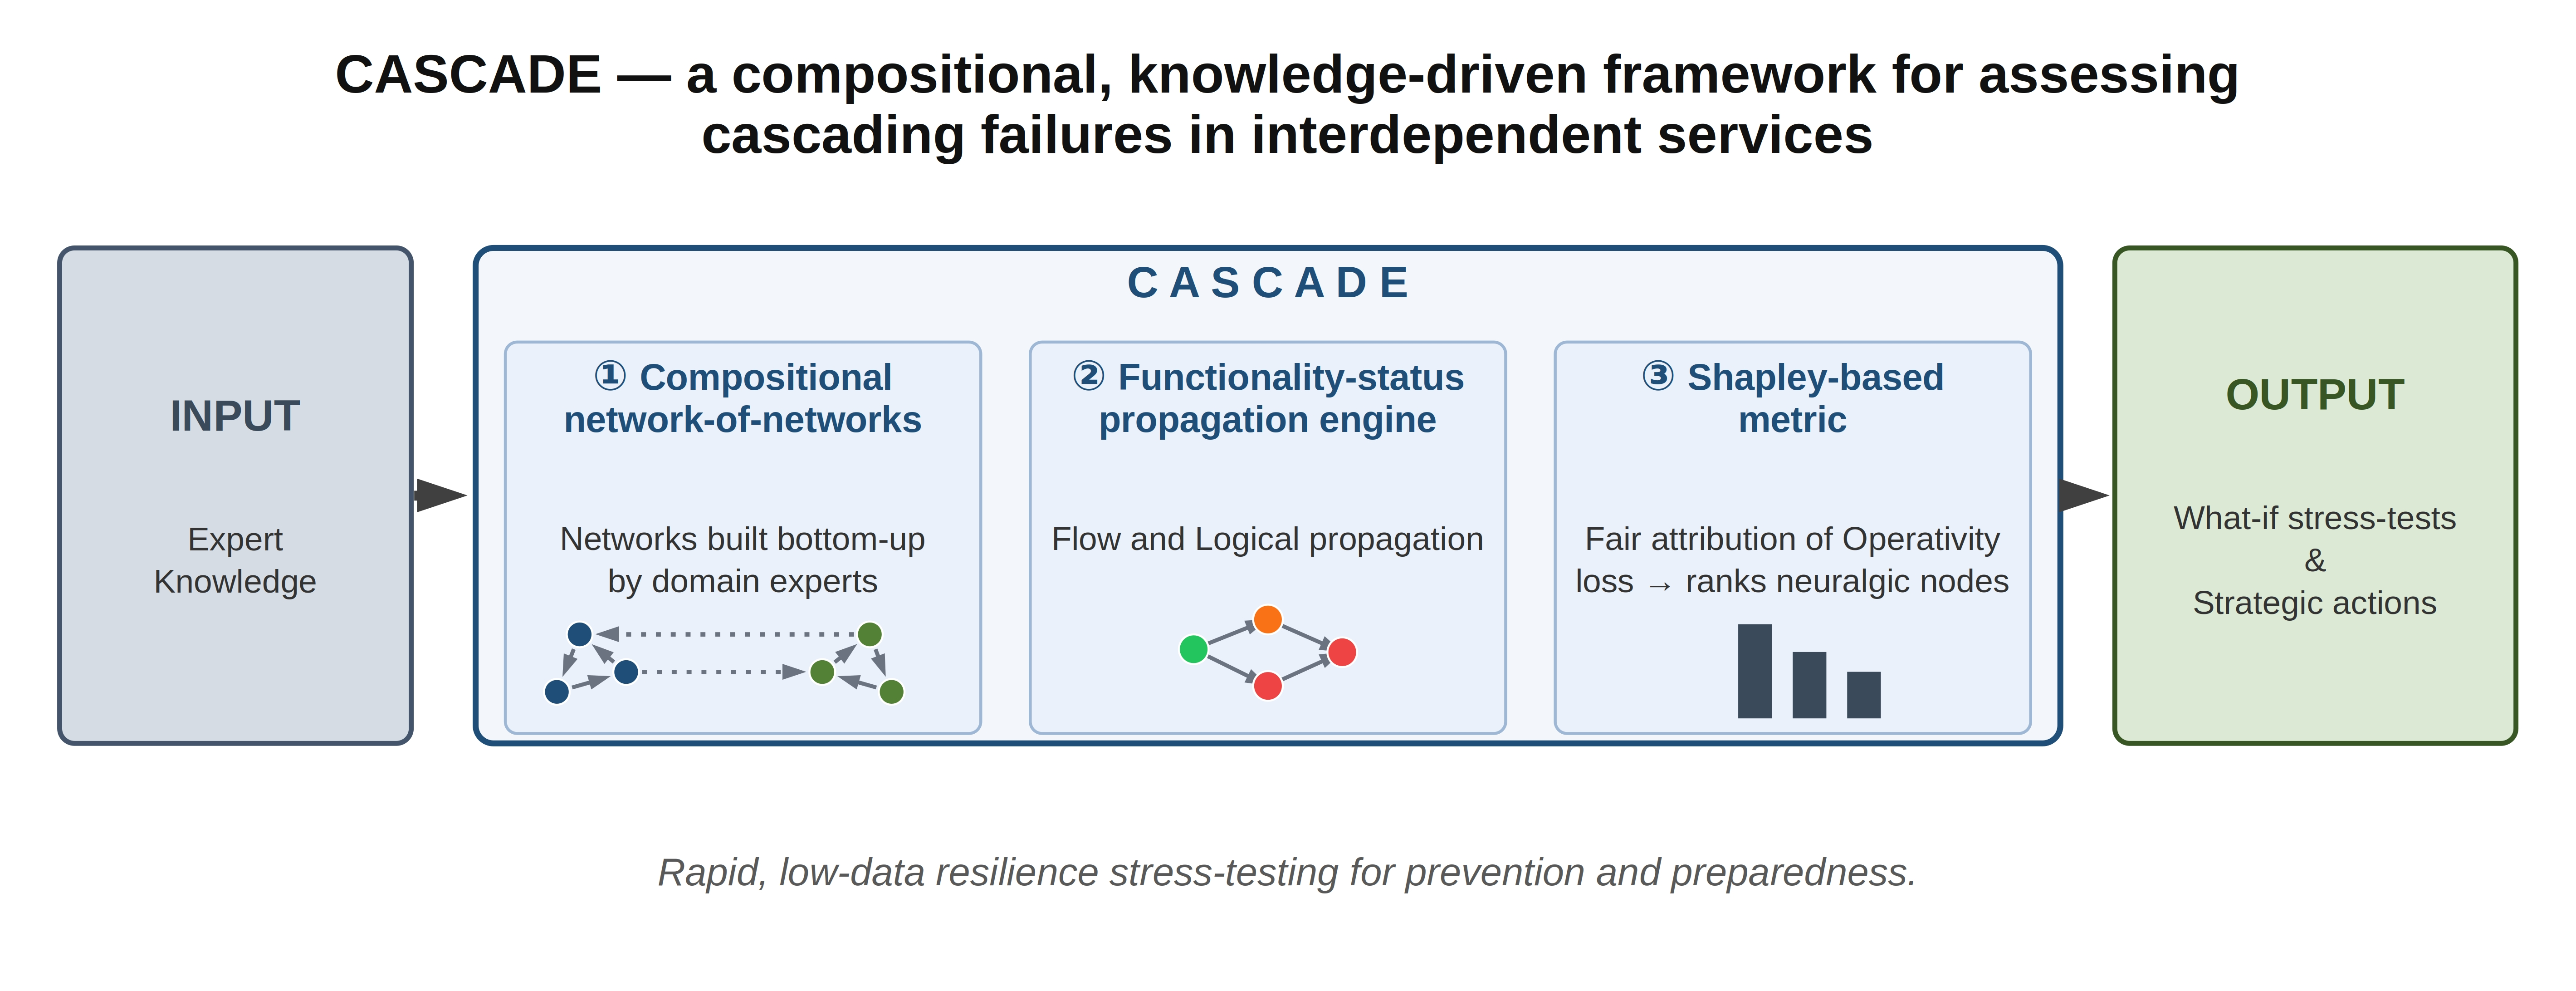
\includegraphics[width=\textwidth]{Figures/CASCADE_graphical_abstract.jpg}
\end{graphicalabstract}

\begin{highlights}
\item CASCADE: open-source framework for cascading failures in interdependent services.
\item Functionality-status propagation engine plus adapted Shapley value node analysis.
\item Rapid, knowledge-based stress-testing for multi-hazard essential-service resilience.

\end{highlights}

\begin{keyword}
Cascading failures \sep Interdependent infrastructure \sep Resilience \sep Decision support \sep Network-of-networks \sep Operativity
\end{keyword}



\end{frontmatter}

\section{Introduction}
\label{sec:intro}

\subsection{The challenge of cascading service failures in disaster scenarios}
\label{subsec:challenge}

Hazards frequently trigger cascading failures across interdependent critical infrastructure systems, amplifying initial damage and prolonging service disruptions. Recent climate-related and systemic events illustrate how strongly coupled infrastructures can transform a localised hazard into a prolonged disaster, severely affecting essential services for millions of people. For example, Hurricane Maria's impact on Puerto Rico in 2017 exposed how interdependencies among power, water, telecommunications, and healthcare systems drove a long-lasting service crisis, ultimately contributing to severe socioeconomic secondary impacts, including huge forced displacement \cite{hurricane_maria, der_sarkissian_investigating_2022}. More recently, the April 2025 blackout across Spain and Portugal demonstrated how disturbances in the interconnected European power system can rapidly propagate through transmission networks, disrupting transport and digital services at a national scale \cite{panel2025grid}. Managing such cascading effects has become a central challenge for modern infrastructure governance. Consequently, the United Nations Office for Disaster Risk Reduction (UNDRR) \textit{Handbook for Implementing the Principles for Resilient Infrastructure} \cite{UNDRR2023Handbook} establishes core guidelines to actively manage ``the interdependent nature of infrastructure and services, or the increasingly complex nature of risks and the cascading impacts that a disaster can have across the whole infrastructure system.'' Global and regional policy frameworks are increasingly reflecting this systemic, intersectoral view. The Sendai Framework for Disaster Risk Reduction 2015--2030 emphasises a cyclical ``understand--govern--invest--prepare'' approach, setting explicit targets to reduce infrastructure damage and essential service disruptions. Furthermore, recent European directives (e.g., \href{https://eur-lex.europa.eu/eli/dir/2022/2557/}{EU 2022/2557}) represent both a consolidation and a paradigm shift: moving from merely protecting physical ``critical infrastructures'' toward guaranteeing the continuity of ``essential services''. This acknowledges that resilience is fundamentally a system-of-systems challenge involving intersectoral organisational governance, where the human factor is key. Building on this evolution, the \href{https://echo-horizon.eu/}{ECHO} European project (Empowering and Connecting Diverse Communities for Multi-Hazard Resilience with Open Data, Open Models, and Open-Source Software) supports a bottom-up, service-centric governance. Under this paradigm, local authorities, essential service providers, and emergency managers co-produce resilience strategies. This localised approach aligns with frameworks such as the UNDRR \href{https://www.preventionweb.net/publication/how-make-cities-more-resilient-handbook-local-government-leaders-2017#downloads}{``10 Essentials for Making Cities Resilient.''} It empowers communities to operationalise national guidelines through integrated data, transparent modelling, and shared operational awareness.

\subsection{Operational needs for accessible cascade analysis}
\label{subsec:operational_need}
Despite recent policy advances, a persistent gap separates conceptual insight from practical tools usable by emergency managers, infrastructure operators, and community stakeholders. Here we recognise three core operational needs.

First, \emph{compositional, cross-sector modelling}. Disaster response is inherently intersectoral, yet utilities, communication and digital service providers, and healthcare typically reason over isolated models of their own systems \cite{ouyang_review_2014,UNISDR2015Sendai}. Practice therefore needs a framework that supports bottom-up construction, letting domain experts develop subsystems independently and subsequently link them into a shared representation that establishes common situational awareness across organisations.

Second, \emph{low data intensity}. Extensive historical records for calibration and validation are frequently unavailable---particularly in developing or resource-constrained regions---and, where they exist, are often fragmented across public and private entities constrained by security, privacy, and institutional data-sharing barriers \cite{balakrishnan_infrarisk_2022,Barriers_data_sharing,data_sharing_fundamentals}. A usable tool must therefore deliver actionable insight from the knowledge operators already hold, rather than presupposing rich, network-specific datasets.

Third, \emph{accessibility to non-specialists}. Much of the knowledge that actually governs system operativity during a crisis---informal heuristics, undocumented workarounds, backup procedures---lives with infrastructure operators and local emergency managers, not with modelling specialists. A tool must make it possible for these stakeholders to encode and interrogate that knowledge directly, without advanced proficiency in network science, probabilistic risk assessment, or software engineering.

These needs carry tangible governance weight. Smaller municipalities and resource-constrained nations often lack the financial and technical capacity to acquire, operate, and continuously update sophisticated simulation platforms \cite{UNDRR2022GAR}, leaving a critical gap between the scientific understanding of hazard-induced cascading failures and the decision-support tools available to those responsible for safeguarding essential services. Meeting the three needs above---compositional modelling, low data requirements, and stakeholder accessibility---is the design target that motivates the research questions set out next.

\subsection{Research questions}
\label{subsec:RQs}
This paper addresses the needs identified above by introducing CASCADE (Customizable Assessment of System Cascades And Dependency Effects), a new methodology and prototype software designed to meet them while maintaining scientific rigour. Each of the three operational needs of Section~\ref{subsec:operational_need} motivates one research question:

\paragraph{RQ1} Given that formal data are scarce and operational knowledge is dispersed across organisations, can a \textbf{compositional} approach let stakeholders model their subsystems independently and integrate them into a shared network-of-networks that captures cross-sector cascading dynamics?

\paragraph{RQ2} Given that preparedness depends on knowing global and complex dynamics, can the modelling process itself \textbf{expand operators' understanding}---revealing dependencies, blind spots, and plausible failure sequences---rather than acting as a black-box calculator?

\paragraph{RQ3} Can a framework support rapid \textbf{stress-testing} of "what-if" situations (e.g.\ upgrading interventions, joint failures), letting stakeholders assess strategic investment and preparedness in an anticipatory approach?


\subsection{Paper organisation}
\label{subsec:organisation}
The remainder of this paper is organised as follows. Section~\ref{sec:litreview} briefly reviews the literature on existing methodologies covering cascading failures in interdependent networks, resilience assessment in graphs, decision support systems for DRR,  and participatory approaches, ultimately positioning CASCADE within this landscape. Section~\ref{sec:cascade_context} presents the CASCADE framework, including its modelling workflow, the functionality-status propagation engine, and the Shapley-based neuralgic node analysis. Section~\ref{sec:case} demonstrates the approach through a realistic case study. Section~\ref{sec:discussion} discusses methodological contributions, practical implications, limitations, and future research directions. Finally, Section~\ref{sec:conclusion} concludes with recommendations for research and practice.

\section{Review of existing approaches}
\label{sec:litreview}
This section examines established approaches for analysing cascading failures in interdependent infrastructures, ranging from quantitative network modelling to participatory governance frameworks. We reflect on the potentialities and limitations of these recognised methodologies to identify the gaps in disaster risk reduction \cite{zio2016challenges, brunner_understanding_2024} that the CASCADE framework seeks to address.

\subsection{Cascading failures in interdependent infrastructure networks}
\label{subsec:cascades}
Foundational research on interdependent infrastructure systems \cite{Rinaldi2002_Interdependencies, Rinaldi2004ModelingAS} established the seminal classification of interdependencies into physical, cyber, geographic, and logical dimensions. Subsequent advancements in Network-of-Networks (NoN) paradigms \cite{buldyrev_catastrophic_2010, Gao2012_NaturePhysics, aleta_multilayer_2026} offer a comprehensive theoretical grounding for understanding cascade dynamics. Crucially, these topological studies demonstrate that even weak inter-system couplings can trigger first-order phase transitions resulting in sudden, catastrophic system collapse rather than gradual operativity degradation. 

More recent literature has sought to refine these classifications to support operational governance better. For instance, Shamsi et al. \cite{shamsi2025interdependency} developed a unified framework that organises dozens of interdependency types across diverse infrastructure sectors. This provides a highly granular vocabulary for describing how essential services rely on one another, fostering shared situational awareness among stakeholders. However, while these taxonomies improve conceptual understanding, translating complex NoN vulnerabilities into actionable intersectoral safety strategies remains a persistent challenge for disaster risk reduction practitioners \cite{Pescaroli2018}.

\subsection{Quantitative resilience assessment via graph modelling}
\label{subsec:graph}

Graph-theoretic approaches remain a cornerstone of quantitative resilience assessment for critical infrastructures (CIs), providing computationally efficient tools to analyse and prioritise vulnerabilities. A substantial body of research utilises topology-based metrics (improving and specialising standard ones such as betweenness and eigenvalue centrality) to assess the relative importance of components \cite{WANG2021100459, Survey_centrality_hypergraphs}, optionally with labelled nodes/edges. In these models, resilience is often equated with structural connectivity or efficiency; critical nodes are identified as those whose removal causes the most significant fragmentation or hinders an aggregated measure such as average shortest path. While these measures offer rapid, data-parsimonious proxies for vulnerability, they cannot provide essential information about the flow of real CIs and service capacities that govern real-world infrastructure operations \cite{hines_topological_2010}, \cite{ouyang2013comparisons}, \cite{bachmann_survey_2020}.

Recent scholarship has increasingly pivoted towards performance-based and dynamic graph modelling to address these limitations. De Marco et al. \cite{DeMarco2025} classify purely topological approaches as useful screening tools for structural vulnerability but emphasise that they are insufficient for quantifying resilience. To bridge this gap, modern frameworks integrate graph topology with functional/flow models to capture cascading failures and restoration trajectories. For instance, Ouyang and Wang \cite{OuyangWang2015} quantify resilience as the ratio of realised to target performance over time, utilising optimisation algorithms to schedule restoration in interdependent systems. Such performance-based and optimisation-based models, however, require hazard-specific fragility curves, physical flow solvers (e.g.\ DC power flow, maximum-flow gas models) calibrated per sector, and genetic-algorithm search over simulated damage scenarios to schedule restoration --- a data and compute-intensive pipeline that De Marco et al.'s own SWOT analysis \cite{DeMarco2025} flags as a recurring weakness of both approach families. CASCADE instead trades this physical fidelity for a lightweight, rule-based heuristic pipeline (Section~\ref{subsec:propagation_engine}) that lets domain experts encode the same restoration and redundancy logic directly as qualitative dependency levels and rules, without fitting per-sector physical models or running scenario-search optimisations.

\subsection{Decision support systems for disaster management}
\label{subsec:dss_twins}
We can distinguish decision support systems (DSS) for disaster management into three broad paradigms: AI-driven analytics, high-fidelity digital twins (DTs), and geographic information system (GIS) based frameworks. Machine learning and AI approaches can process large spatiotemporal datasets to anticipate hazard trajectories and improve situational awareness, yet they often rely on extensive labelled data (frequently unavailable across jurisdictions) and may introduce ``black-box'' opacity that undermines accountability and uptake \cite{Kyrkou2023,karunakaran_ai-driven_2025}. At the other end of the spectrum, GIS-centric tools remain widely adopted because they are comparatively transparent, less resource-intensive, and well-suited to eliciting and formalising expert tacit knowledge, particularly in data-scarce settings \cite{adu2025role}. However, such tools typically provide limited support for dynamic simulation, thereby struggling to represent temporal dependencies, cross-sector feedbacks, or flow-based service logic.

DT technologies sit between these extremes and are increasingly recognised as a potentially transformative paradigm for infrastructure resilience. By coupling real-time sensor streams with simulation models, DTs provide dynamic virtual representations that enable continuous monitoring, forecasting, and the testing of response strategies in a risk-free environment, including ``what-if'' analyses of cascading infrastructure failures \cite{Inyang2024,Kaveh_Alhajj_2025,Afolabi2025,Zhu2025}. Despite this promise, operational adoption remains uneven and is often confined to high-value assets or research pilots, largely due to substantial development and maintenance costs, computational demands, and the technical difficulty of integrating heterogeneous, fragmented data sources \cite{Inyang2024,Karaduman2025}. Interoperability barriers, driven by proprietary formats and siloed governance, further constrain the seamless information flow required for holistic and cross-sector resilience planning \cite{Afolabi2025}. These limitations are motivating a shift towards hybrid DSS architectures that integrate DT-based simulation with explainable AI (XAI) and human-in-the-loop mechanisms within familiar, map-centred interfaces, aiming to balance analytical power with usability, transparency, and user trust \cite{Domfeh2025}. In parallel, recent research advocates federated ``system-of-systems'' approaches that decompose complex infrastructures into modular, communicating twins rather than monolithic models, improving scalability while better reflecting real-world institutional fragmentation. Building on this trajectory, the emerging concept of ``Digital Risk Twins'' focuses explicitly on disaster management, emphasising human-in-the-loop designs that combine automated sensing with expert judgement to cope with the uncertainty and time pressure that characterise emergency response \cite{ghaffarian_rethinking_2025}.



\subsection{Qualitative approaches and participatory resilience} \label{subsec:qualitative} Parallel to the advancement of quantitative models, a paradigm shift towards qualitative and participatory methodologies has emerged, acknowledging that resilience is also fundamentally a socially constructed and context-dependent phenomenon. While quantitative metrics capture structural capacity, qualitative investigations through semi-structured interviews, focus groups, or grounded theory are essential for elucidating the \textit{human dimensions} of resilience, including risk perception, trust in governance, and informal coping heuristics that dictate actual system behaviour during crises \cite{Aldunce2015_Resilience, BraunClarke2006}. To bridge the gap between technical assessments and local realities, Participatory GIS (PGIS) \cite{McCall2003} and Q-methodology\cite{lundberg2020} have gained prominence as tools to formalise tacit knowledge. These methods allow communities to spatially visualise vulnerabilities and rank resilience priorities, revealing socio-spatial inequalities that aggregate statistical models frequently overlook \cite{Cadag2012_PGIS, Ma2024}. Institutional frameworks have increasingly codified these bottom-up principles to support decentralised governance. The Community-Based Disaster Risk Management (CBDRM) paradigm and the UNDRR's Ten Essentials for Making Cities Resilient'' explicitly position local stakeholders not merely as beneficiaries, but as active co-producers of safety strategies, emphasising the critical role of social capital—bonding, bridging, and linking—in disaster recovery \cite{UNDRR2023Handbook, Shaw2012}. Similarly, the \href{https://www.rockefellerfoundation.org/}{Rockefeller Foundation's 100 Resilient Cities (100RC)} initiative attempted to institutionalise this holistic view through Chief Resilience Officers and multi-stakeholder strategies. However, the operationalisation of these frameworks remains fraught with challenges regarding power dynamics and genuine inclusion \cite{Spaans2017,Hofmann2021}. Furthermore, a persistent methodological divide exists: qualitative insights are rarely integrated into tools for strategic decisions, creating a disconnection between the expert understanding of resilience and the technical governance of essential services.


\subsection{Synthesis: gaps in current approaches}
\label{subsec:gaps}

Read against the operational needs of Section~\ref{subsec:operational_need},
the reviewed strands leave four recurring gaps.

\begin{itemize}
  \item \textbf{Topology doesn't grasp functional dynamics.} Graph and network-of-networks models
  (Sections~\ref{subsec:cascades},~\ref{subsec:graph}) offer accessible, data-parsimonious
  common ground, but being largely topological they miss crucial phenomena that govern real operativity.

  \item \textbf{Accessibility versus fidelity.} Full digital twins and physics-based simulations (Section~\ref{subsec:dss_twins}) capture such dynamics but are costly, data-hungry, and expertise-intensive, hence rarely deployable in resource-constrained
  settings.

  \item \textbf{Missing temporal dynamics.} Most methods assess static snapshots, yet
  backup exhaustion, time-limited redundancy, and recovery sequencing---decisive for whether
  a cascade is contained---are inherently temporal.

  \item \textbf{Completeness versus tractability.} Exhaustive analysis of interdependent
  failures is computationally demanding at realistic scale, so usable tools need principled,
  interpretable approximations.
\end{itemize}

Moreover, the tacit operational knowledge needed to close these gaps already exists among
operators and emergency managers (Section~\ref{subsec:qualitative}) but is seldom captured in
a form quantitative tools can use. CASCADE targets this niche: composable cross-sector models
built from expert knowledge, with explicit temporal and backup dynamics, tractable enough for
practical use.



\section{The CASCADE framework}
\label{sec:cascade_context}

CASCADE was developed following a Rapid Application Development (RAD) methodology \cite{Beynon-Davies01091999}---emphasising iterative prototyping and continuous user involvement over rigid upfront specification. Rather than assuming requirements can be fully fixed before implementation, we produced functional prototypes early, presented them to practitioners and emergency experts, and refined the framework from their feedback. This kept CASCADE aligned with real operational needs and its core concepts intuitive to non-technical users.

This section first describes what CASCADE is (Section~\ref{subsec:what_cascade_is}), then guides the reader through how it is used in practice (Section~\ref{subsec:how_cascade_is_used}), and finally, for completeness, details the technical methodology of the propagation engine (Section~\ref{subsec:propagation_engine}) and the Shapley-based analysis (Section~\ref{subsec:shapley}).


\subsection{What CASCADE is}

\begin{figure}
    \centering
    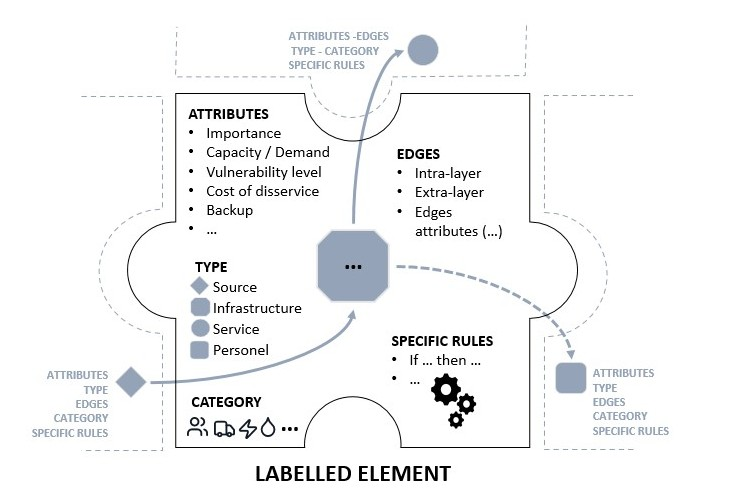
\includegraphics[width=0.7\linewidth]{Figures/puzzle.jpg}
    \caption{\textbf{Schema of a labelled element in CASCADE}. Every node is depicted as a puzzle piece to emphasise that it interlocks with its neighbours through composable connections. An element declares a \texttt{Type} (source, infrastructure, service, or personnel, distinguished by shape) and one or more \texttt{Category} (e.g.\ electric, water, transport, managerial) identifying the service it provides. \texttt{Attributes} (e.g.\ capacity/demand, vulnerability level, backup, importance \dots) parametrise its behaviour under stress, while \texttt{Edges} — intra-layer or extra-layer, each carrying its own attributes — record which service flows from one element to another. \texttt{Specific rules} attach optional if--then conditions that override the default propagation logic for this element.
    Because every connected neighbour (dashed outlines) exposes the same schema, a network is built by composing identically structured, self-describing pieces, which is what enables CASCADE's compositional, bottom-up modelling paradigm.}
    \label{fig:puzzle}
\end{figure}
\label{subsec:what_cascade_is}

CASCADE (Customizable Assessment of System Cascades And Dependency Effects) is
a knowledge-driven framework for exploring how disruptions and disservices
propagate through interconnected services and infrastructures. Rather than
starting from measurements or historical datasets, it starts from what
operators and planners already know about their systems: who depends on whom,
what redundancies exist, and how long backups last. Our approach turns this
knowledge into a structured, analysable network which guides the users to
surface inconsistencies, missing information, and divergent assumptions.

Conceptually, CASCADE represents an interdependent system as a directed graph
of nodes and edges. Nodes represent sources, infrastructures\footnote{more generally, an "infrastructure" node can also represent equipment or devices.}, personnel or services; edges represent the provision of any service/utility from the tail node to the head node, hence modelling the dependency.
Each node and each edge is associated with a \emph{Functionality} value drawn
from a discrete integer scale $1\ldots N$ (1\,=\,worst, $N$\,=\,fully
operational), configured per project (the default sets $N=3$, with labels
\texttt{critical}, \texttt{operational\_warning}, and \texttt{operational}),
which is used to express degradation under hazards or under internal and
external disservices. An orthogonal \emph{Functionality Time} attribute (a
countdown in hours) can be attached to any element to signal that it is
temporarily holding its current Functionality against an ongoing shortfall and will drop to the worst level once the countdown expires.
Nodes and edges can be annotated with a rich set of attributes: vulnerability levels on hazards or external services, dependency profiles on modelled services, time-limited backups (with associated durations), and numerical values such as demand or capacity where relevant. Additional socio-economic attributes, such as importance or cost of disservice, can be attached to support the interpretation and prioritisation of results.

To model emergency scenarios, CASCADE supports stress-testing the system against different hazards, external disservices, or more general functionality-degradation scenarios.

A propagation engine updates node/edge Functionality values (also advancing Functionality Time countdowns via explicit temporal jump events) according to a propagation engine, revealing how local disruptions can evolve into complex, multi-step cascades that would be difficult to track mentally. The resulting trajectories and summaries highlight components that are neuralgic for keeping essential services operational. We call a node \emph{neuralgic} when many other services depend on it, so that its degradation propagates widely through the network. Users can then refine the model and immediately explore the impact, for instance, by adding or relocating backups and revising dependencies. Because the underlying model is explicit and editable, users can easily adjust element attributes and immediately explore the implications of proposed policy changes or interventions.

To summarise the effect of a scenario in a single figure, CASCADE computes an \emph{Operativity Score}: a weighted, normalised average of node Functionalities, expressed as a percentage of the fully operational state,
\[
  \Omega(s) \;=\; 100 \times
  \frac{\sum_{i} w_i\, f_i(s)}{N \sum_{i} w_i}\,,
\]
where $f_i(s)\in\{1,\ldots,N\}$ is the Functionality of node $i$ in state $s$ and
$w_i \ge 0$ its weight. The weighting is user-selectable, so the same network can
be scored from different governance viewpoints:
\begin{itemize}
  \item \emph{Equal weight} ($w_i = 1$): every node counts the same---a purely topological reading of how much of the system remains operational;
  \item \emph{Importance} ($w_i = \mathrm{importance}_i$): a user-assigned criticality value, letting strategic assets (e.g.\ a hospital) dominate the score;
  \item \emph{Cost of disservice} ($w_i = \mathrm{cost\_of\_disservice}_i$): the economic or social cost incurred per unit time while node $i$ is down, aligning the score with expected loss rather than node count.
\end{itemize}
Because the Shapley analysis (Section~\ref{subsec:shapley}) defines the value of a failure coalition as the resulting drop in $\Omega$, the choice of weighting directly shapes which elements are deemed neuralgic.

\subsection{How CASCADE is used in practice}
\label{subsec:how_cascade_is_used}


From a user's viewpoint, CASCADE is software designed to support an intuitive, iterative workflow rather than a one-off modelling exercise.
See Figure~\ref{fig:CASCADEworkflow} for a visual summary of the workflow described in the following.

\paragraph{Modelling the system as a multi-labelled graph}
Users begin by building a graph/network model of their system. They add nodes for key sources, infrastructures, services, and operators, and connect them with directed dependency edges. Nodes are grouped into categories (e.g.\ electric, water, transport, manager), which later determine how propagation is handled by correctly interpreting redundant services. For each node, users can set a per-category dependency level that controls how strongly an upstream degradation in that category propagates to the node, and can enable a time-constrained backup for any category.

\paragraph{Encoding operational knowledge as rules}
CASCADE allows users to formalise operational knowledge as explicit if--then, intercategorical and intracategorical rules that modify or complement the default propagation behaviour. Rules can target both nodes and edges, and their conditions can refer to any attribute of the involved elements (e.g.\ any custom attribute added), though by default they are based on Functionality values. Intracategorical rules describe how multiple predecessors within the same category interact to serve a target node (e.g.\ redundant feeds), while intercategorical rules describe how different services jointly determine a node's Functionality (e.g.\ a hospital requiring both electricity and road access). Because rules are written in a strict but readable form, users can inspect, discuss, and revise them.

\paragraph{Running stress tests and exploring scenarios}
Once the network topology, attributes and operational rules are established, users can simulate systemic stress by defining hazards or localized disruptions to selected nodes or edges. CASCADE models the subsequent impact propagation, illustrating the progressive degradation of system operativity. This comparative capability allows users to evaluate how varying hazard parameters or policy interventions influence cascade trajectories. Consequently, the software facilitates the discovery of emergent, unanticipated disaster scenarios. To exploit CASCADE fully, users benefit from a proactive mindset. Traditional Failure Mode and Effects Analysis (FMEA~\cite{huang_failure_2020}) asks ``how can this component fail?'' and traces the effects forward. CASCADE rewards the complementary, anticipatory stance of Anticipatory Failure Determination (AFD)~\cite{da_silva_anticipatory_2019, zio2016challenges}: starting from an undesired outcome---the loss of a critical service---and working backwards to uncover the conditions and combinations of failures that could bring it about. By systematically hypothesising these failure pathways, users surface non-obvious vulnerabilities before a hazard does, so they can be anticipated and prevented.

\paragraph{Interpreting results and iterating}

CASCADE summarises system behaviour through customizable Operativity Score and provides graphical overviews of each scenario by showing directly affected elements, immediate propagation effects, and the situation after a defined time interval. A game-theoretic analysis module based on Shapley values can rank nodes by their contribution to overall Operativity loss across many combinations of failures, highlighting neuralgic components that may not be obvious from topology-based metrics (which are also available). This supports iterative planning, participatory workshops, and communication with non-expert stakeholders, such as decision-makers responsible for investment and preparedness strategies.

\begin{figure}[H]
    \centering
    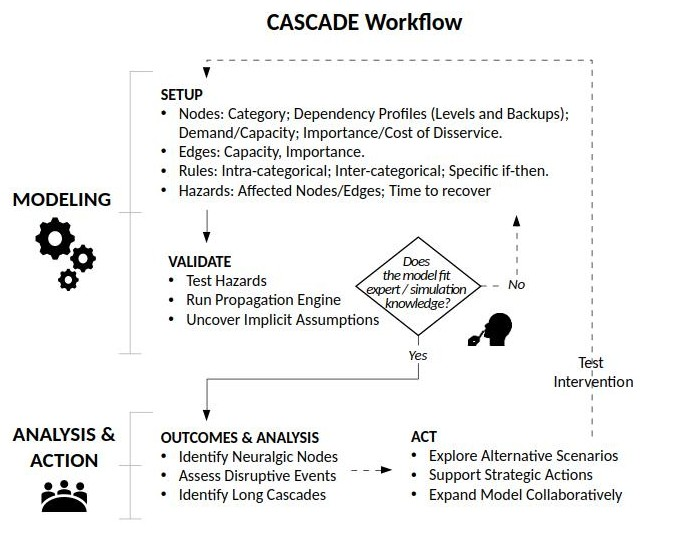
\includegraphics[width=1\linewidth]{Figures/CASCADE Workflow.jpg}
    \caption{The CASCADE workflow. During \textbf{modelling}, the user \emph{sets up}
the system as an interdependent network-of-networks (labelled nodes and edges, operational rules, hazards) and \emph{validates} it by running the propagation engine and comparing the cascades against expert or simulation knowledge---a step that surfaces implicit assumptions and loops back for refinement until the model fits. The validated model then drives \textbf{analysis and action}: identifying neuralgic nodes, assessing disruptive events, and tracing long cascades, then acting on the results by comparing interventions, exploring alternatives, and expanding the network-of-networks as new stakeholders contribute their own subsystems. The outer feedback loop keeps the process iterative and participatory.}

    \label{fig:CASCADEworkflow}
\end{figure}

\subsection{Propagation engine: heuristic pipeline and rule semantics}

\label{subsec:propagation_engine}
\begin{figure}[H]
  \centering
  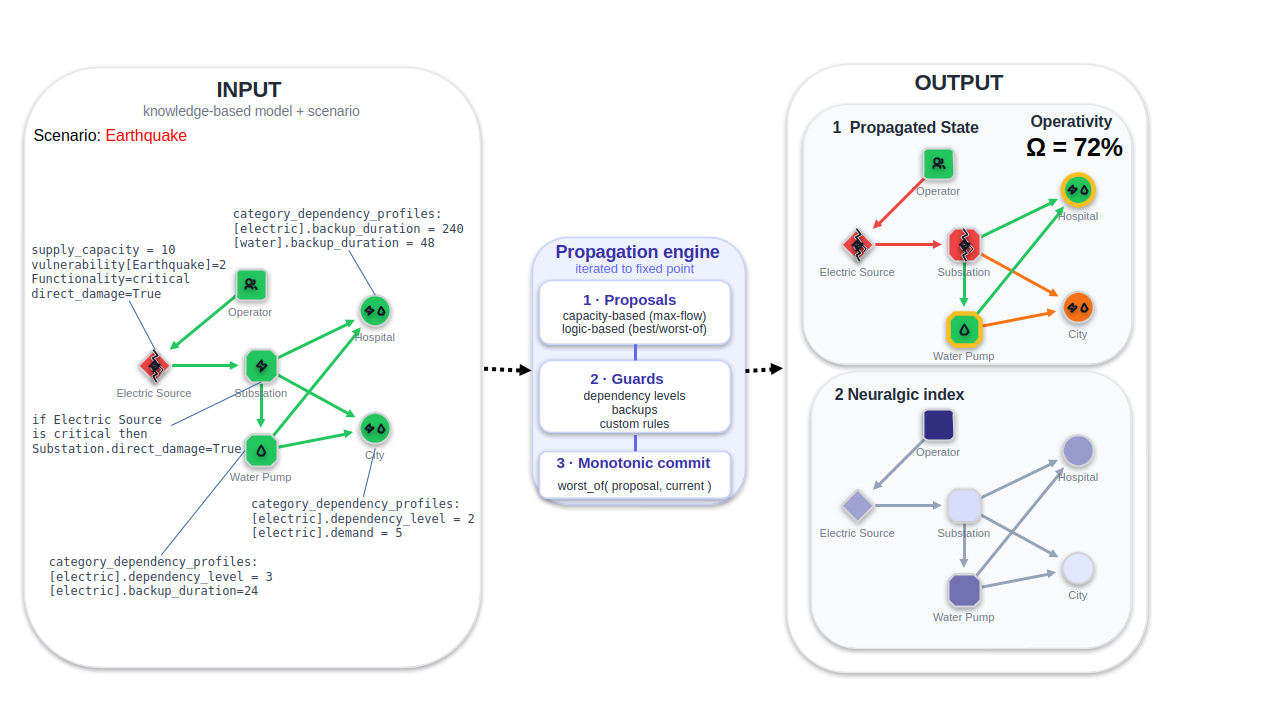
\includegraphics[width=\linewidth]{Figures/anatomy.png}
  \caption{\textbf{Anatomy of a CASCADE analysis}, shown on a minimal
  interdependent network (an electric source and its substation, a water pump,
  a hospital and a city, and the human operator that controls the grid).
  CASCADE represents a system as a directed graph and simulates how a
  disruption \emph{propagates} through it.
  %
  \textbf{Input (left) --- the model and a scenario.}
  Each \emph{node} is a source, infrastructure, service or operator
  (distinguished by shape); the icon(s) inside a node represent the \emph{category}
  of service it provides (electricity, water, operator). A directed
  \emph{edge} $a\!\rightarrow\!b$ reads ``$a$ supplies/enables $b$'', i.e.\ $b$
  depends on $a$. Every node carries a discrete \emph{Functionality}: \emph{critical} as red; \emph{operational\_warning} as orange and \emph{operational} as green.
  Beyond its status, a node carries knowledge-based attributes. A source declares how much it can provide through \texttt{supply\_capacity}, and a consumer how much it needs through \texttt{demand}. For every category it depends on,
  a node sets a \texttt{dependency\_level} which
  tunes how strongly a shortfall in that category drags it down. It may also keep a \texttt{backup} for a given category, a reserve that holds it at its current status for \texttt{backup\_duration} hours after that supply fails.
  Node's exposure to a hazard is represented by the \texttt{vulnerability\_level}, from unaffected to fully degraded. Finally, \texttt{rules} are user-written \texttt{if--then} guards attached to the element they act on.
 The \emph{scenario} initialises the state: an Earthquake sets the \texttt{Electric Source} to
  \emph{critical} via its \texttt{vulnerability\_level} (direct damage is rendered as a crack).
  %
  \textbf{Engine (centre).} The propagation engine iterates to a fixed point. For
  each node it forms a \emph{proposal}, passes it through \emph{guards} (dependency-level attenuation, time-limited backups, and custom rules), and \emph{commits} it monotonically.
  %
  \textbf{Output (right) --- two complementary readings.}
  \emph{(1)~Propagated state}: the cascaded Functionality of every node thorugh the colour code, where an amber ring marks a node currently \emph{holding on
  backup}. Here the blackout criticalises the \texttt{Substation} (the rule
  cracks it representing a physical damage requiring intervention), the \texttt{City} degrades to warning, while the \texttt{Hospital}
  and \texttt{Water Pump} survive on backup; the single-number \emph{Operativity
  Score} $\Omega$ (weighted mean Functionality) summarizes numerically the propagated situation.
  \emph{(2)~Neuralgic index}: a Shapley-value ranking of how much each node's failure contributes to overall operativity loss (darker $=$ more neuralgic).}
  \label{fig:anatomy}
\end{figure}

CASCADE's propagation engine simulates how service disruptions ripple through the interdependent network. Starting from an initial scenario in which specific components have their Functionality degraded, the engine iteratively propagates these effects until the network settles into a new stable state — a fixed point at which no further degradation occurs.
During the cascade, a component's Functionality can only deteriorate or remain unchanged, never autonomously recover. This strict downward progression ensures simulation convergence to a final post-scenario state.

\paragraph{Two category types}
Services provided from nodes are defined by a \textit{category} attribute.
Two category types exist:
\begin{itemize}
  \item \emph{SourceToDemands} categories (e.g., electricity, water) model flow generated by sources, transmitted across the network, and consumed by nodes with a positive demand value.
  \item \emph{Requisite} categories (e.g.,  connectivity, human
    management) represent essential, non-consumable dependencies whose sheer presence or absence dictates a component's operability.
\end{itemize}

\paragraph{Complementary propagation mechanisms}
To accurately reflect these differing realities, the engine combines two complementary mechanisms operating over the same network:
\begin{enumerate}
  \item \textbf{Universal logical propagation:} In every round, the engine runs a logical aggregation pass over every\footnote{Except for those that have a category typed \emph{SourceToDemands} and with every parent node of the same category: this case is handled with the Capacity-based propagation.} node. The aggregation follows two nested rules. First, among all incoming nodes that carry the \emph{same} category, the engine proposes the best available status (i.e., a \texttt{best\_of} across co-category suppliers): a single healthy supplier is sufficient to satisfy the need of the service associated with that category. Second, across \emph{different} categories the engine takes the worst result (i.e., a \texttt{worst\_of} across categories): a node that receives both electricity and water must have both adequately supplied, so a failure in any one category degrades the node. The resulting status is then fed into the monotonic commit step alongside the capacity-based proposal. By running this pass universally, the engine automatically reads the dependency structure from the labelled graph topology itself: a node that happens to receive edges from two different categories is implicitly treated as requiring both, deferring the need for the user to declare an explicit cross-category rule only to change the defaulting behaviour.
  \item \textbf{Capacity-based propagation:} For nodes with positive demand in a \emph{SourceToDemands} category, the engine additionally runs a priority-aware min-cost max-flow pass (\cite{edmonds1972theoretical,orlin1997polynomial,SciPyProceedings_11}) and maps the served ratio to a Functionality proposal. This module captures quantity-dependent flow dynamics---such as partial supply and priority-driven flows---that purely logical dependency models cannot represent faithfully.
\end{enumerate}

Reconciling these heterogeneous mechanisms onto a common functionality-status representation is what makes the engine extensible: because every mechanism ultimately expresses its result as a Functionality value, more sophisticated domain simulations (e.g.\ detailed hydraulic, power-flow, or traffic models) can, as future extension, be wrapped behind the same interface and integrated as additional propagation mechanisms, and made to interact with one
another within a single cascade. Importantly, the scope of this engine is not to provide detailed physical simulations for engineering design, real-time operation, or automated control. Rather, it allows stakeholders to rapidly explore cascading disruption scenarios, adopting a comprehensive, knowledge-based systemic view.

\paragraph{The heuristic pipeline}
After the propagation mechanisms produce a candidate Functionality proposal for each node, the proposal passes through the following guards and commit logic before it is applied:
\begin{enumerate}
  \item \textbf{Dependency and Backup Adjustment:} The proposal is first modulated by the node's specific dependency profile for the relevant category:
    \begin{itemize}
      \item \emph{Dependency Levels:} Each node carries, per category, a dependency level on the same integer scale $1\ldots N$ as Functionality. The level sets how strongly a degradation arriving through that category is allowed to pull the node Functionality down: Level~1 neutralises the category's influence entirely (the node never degrades because of it), Level~$N$ passes the degradation through in full, and intermediate levels attenuate it (e.g.\ softening a \texttt{critical} proposal to an \texttt{operational\_warning}). In practice, this lets a modeller state that, say, a hospital depends only weakly on the road network but critically on electricity, without writing an explicit rule for each case.

      \item \emph{Time-Constrained Backups:} If a node possesses a backup and its Functionality would drop due to the current proposal,  the drop is deferred: the node holds its current Functionality and its Functionality Time is set to the backup duration. The deferred drop is noticeable through a  \emph{Temporal Jump} event that advances simulated time.
    \end{itemize}
  \item \textbf{Specific-Rule Override}\textbf{:} The engine then evaluates user-defined conditional rules that encode policy-level behaviours and workarounds. These take the explicit form:
    \texttt{if} $\langle\text{condition}\rangle$ \texttt{then}
    $\langle\text{target}\rangle$ \texttt{is} $\langle\text{value}\rangle$.
    Conditions are Boolean formulas (\texttt{and}, \texttt{or}, \texttt{not})  evaluating node or edge attributes (generally, Functionality values). If a condition evaluates to true, the rule's consequent value replaces the adjusted proposal, overriding both the dependency attenuation and any
    backup deferral set in the previous step.
  \item \textbf{Monotonic Commit:} Finally, the adjusted proposal is compared against the node's current Functionality using a $\texttt{worst\_of}$ combinator. The system only commits the update if the new value is strictly worse than the current one. This enforces the monotonicity required to guarantee the simulation's mathematical convergence.
\end{enumerate}
The engine iterates the logical and capacity-based mechanisms---alongside this pipeline---until a fixed point is reached where no further element can be worsened.

\subsection{Shapley-based neuralgic node analysis}
\label{subsec:shapley}
Having defined the propagation engine for cascading Functionality updates
%--- FIX 7 ---
(Section~\ref{subsec:propagation_engine}), we further leverage it to identify \emph{neuralgic elements}---nodes and edges whose failure most severely compromises overall system operativity. To achieve this, we adapt the Shapley value~\cite{shapley1953value} from cooperative game theory, providing a principled method to quantify each component's contribution to the continuity of essential services across the network.

\subsubsection{Formulating failure as a cooperative game}
\label{subsubsec:shapley_game}
In this framework, the network elements (nodes and edges) are interpreted as ``players'' in a cooperative game, and a ``coalition'' represents a specific combination of elements failing simultaneously. The ``value'' of any such coalition is defined as the resulting \emph{drop in the overall system Operativity Score}, which is computed by running the propagation engine from the current Scenario to its cascaded fixed point.

Crucially, this analysis is not restricted to a fully operational baseline. The assessment can be initialised from \emph{any} network state, including one already degraded by an ongoing hazard or prior cascade. In these cases, the analysis quantifies the \emph{additional} vulnerability introduced by the remaining operational elements, supporting dynamic prioritisation in "what-if" situations.

In classical terms, a component's Shapley value represents its average marginal contribution to all possible coalitions; in the context of CASCADE, it quantifies an element's ``fair share'' of the total operativity loss across all potential failure scenarios. Conceptually, if we imagine infrastructure components failing one by one in a random sequence, each component's failure causes a specific drop in system operativity, and the Shapley value of an element is its average operativity drop calculated across all possible failure sequences. It guarantees that the total vulnerability of the system is fairly distributed among its constituent parts, properly accounting for complex interaction effects, redundancies, and cascading dependencies.

\subsubsection{Achieving computational tractability}
\label{subsubsec:shapley_approx}
Computing exact Shapley values requires evaluating every possible combination of component failures, leading to an exponential computational cost. To make this analysis computationally practical, CASCADE employs a sampling-based approximation strategy governed by three user-configurable constraints:
\begin{itemize}
  \item \textbf{Monte Carlo permutation sampling:} Rather than evaluating all possible failure sequences, the algorithm samples a subset of $M$ random permutations. As $M$ increases, the estimated Shapley values converge toward their exact theoretical expectations.
  \item \textbf{Coalition size truncation:} The analysis introduces a user-defined limit ($k_{\max}$) on the maximum number of concurrent failures considered. This restricts the depth of the search space to a computationally manageable size, motivated by the practical observation that the most critical, actionable vulnerabilities typically emerge from relatively small combinations of concurrent failures.
  \item \textbf{Wall-clock time budget:} A user-specified time limit
    terminates sampling once elapsed computation time exceeds a defined threshold, ensuring responsiveness in interactive sessions even for large networks. Shapley values are reported from however many permutations were completed within the budget.
\end{itemize}

\subsubsection{Actionable outputs}
\label{subsubsec:shapleyoutputs}
Because every sampled failure scenario is evaluated using CASCADE's core propagation engine, the resulting Shapley values intrinsically account for resource flows, logical dependencies, user-defined rules, and backup system dynamics. Consequently, the analysis generates highly actionable outputs, such as:
\begin{itemize}
  \item \emph{Neuralgic element rankings:} Identifying nodes and edges that are functionally vital, including those that may not appear structurally central in standard topological assessments.
  \item \emph{Redundancy validation:} Revealing structurally prominent
    components that actually possess low Shapley values due to effective backup mechanisms or alternative routing, thereby preventing misdirected mitigation investments.
  \item \emph{Hidden joint vulnerabilities:} Identifying small combinations of elements whose isolated failures may be safely absorbed by the system, but whose concurrent failure triggers catastrophic service loss.
\end{itemize}




\section{CASCADE Demonstration Through a Case Study}
\label{sec:case}



\subsection{Modelling Interdependent Urban Services}
\label{subsec:case_modelling}

The demonstration network is a synthetic yet realistic multi-layered network representing a medium-sized multi-urban context with electric power, water, transport, and organisational layers.
The network comprises \textbf{39 nodes} and \textbf{93 directed edges}, distributed across five layers (Electrical, Water, Transport, Managerial, and Service) with inter-layer edges dashed in Figure~\ref{fig:layers_all}. Realistic redundancies, backup buffers, and vulnerability profiles are compiled with a mixture of existing online resources (\href{https://openinframap.org/about}{Openinframap}, \href{https://eaglefvg.regione.fvg.it/}{Eaglefvg}), the author's territorial knowledge, and informed by brief, informal feedback from operators; this feedback was not a structured empirical validation protocol, and the case study should be read as a proof-of-concept demonstration rather than a validated model (see Section~\ref{subsec:limitations}). All network maps in this section follow the legend detailed in Figure~\ref{fig:map_legend}.

\paragraph{Electric subsystem}
A single high-level source (\texttt{Electric Source},
$\mathit{supply\_capacity} = 100$) feeds eight distribution substations
(\texttt{Palmanova electric}, \texttt{Sud electric},
\texttt{San Marco electric}, \texttt{Jalmicco electric},
\texttt{Joint est electric}, \texttt{Industrial electric},
\texttt{Sottoselva electric}, \texttt{Est electric}),
which in turn supply municipal service and essential-service nodes through
directed edges.
The \texttt{power} category is typed \texttt{SourceToDemands}, so when supply
falls short of aggregate demand the engine allocates available capacity through
priority-weighted min-cost max-flow.
The Electric Source carries a \texttt{manager} dependency (dependency level~2):
digital control by the \texttt{electric Operator} is required for safe
management.
\begin{figure}[H]
  \centering
  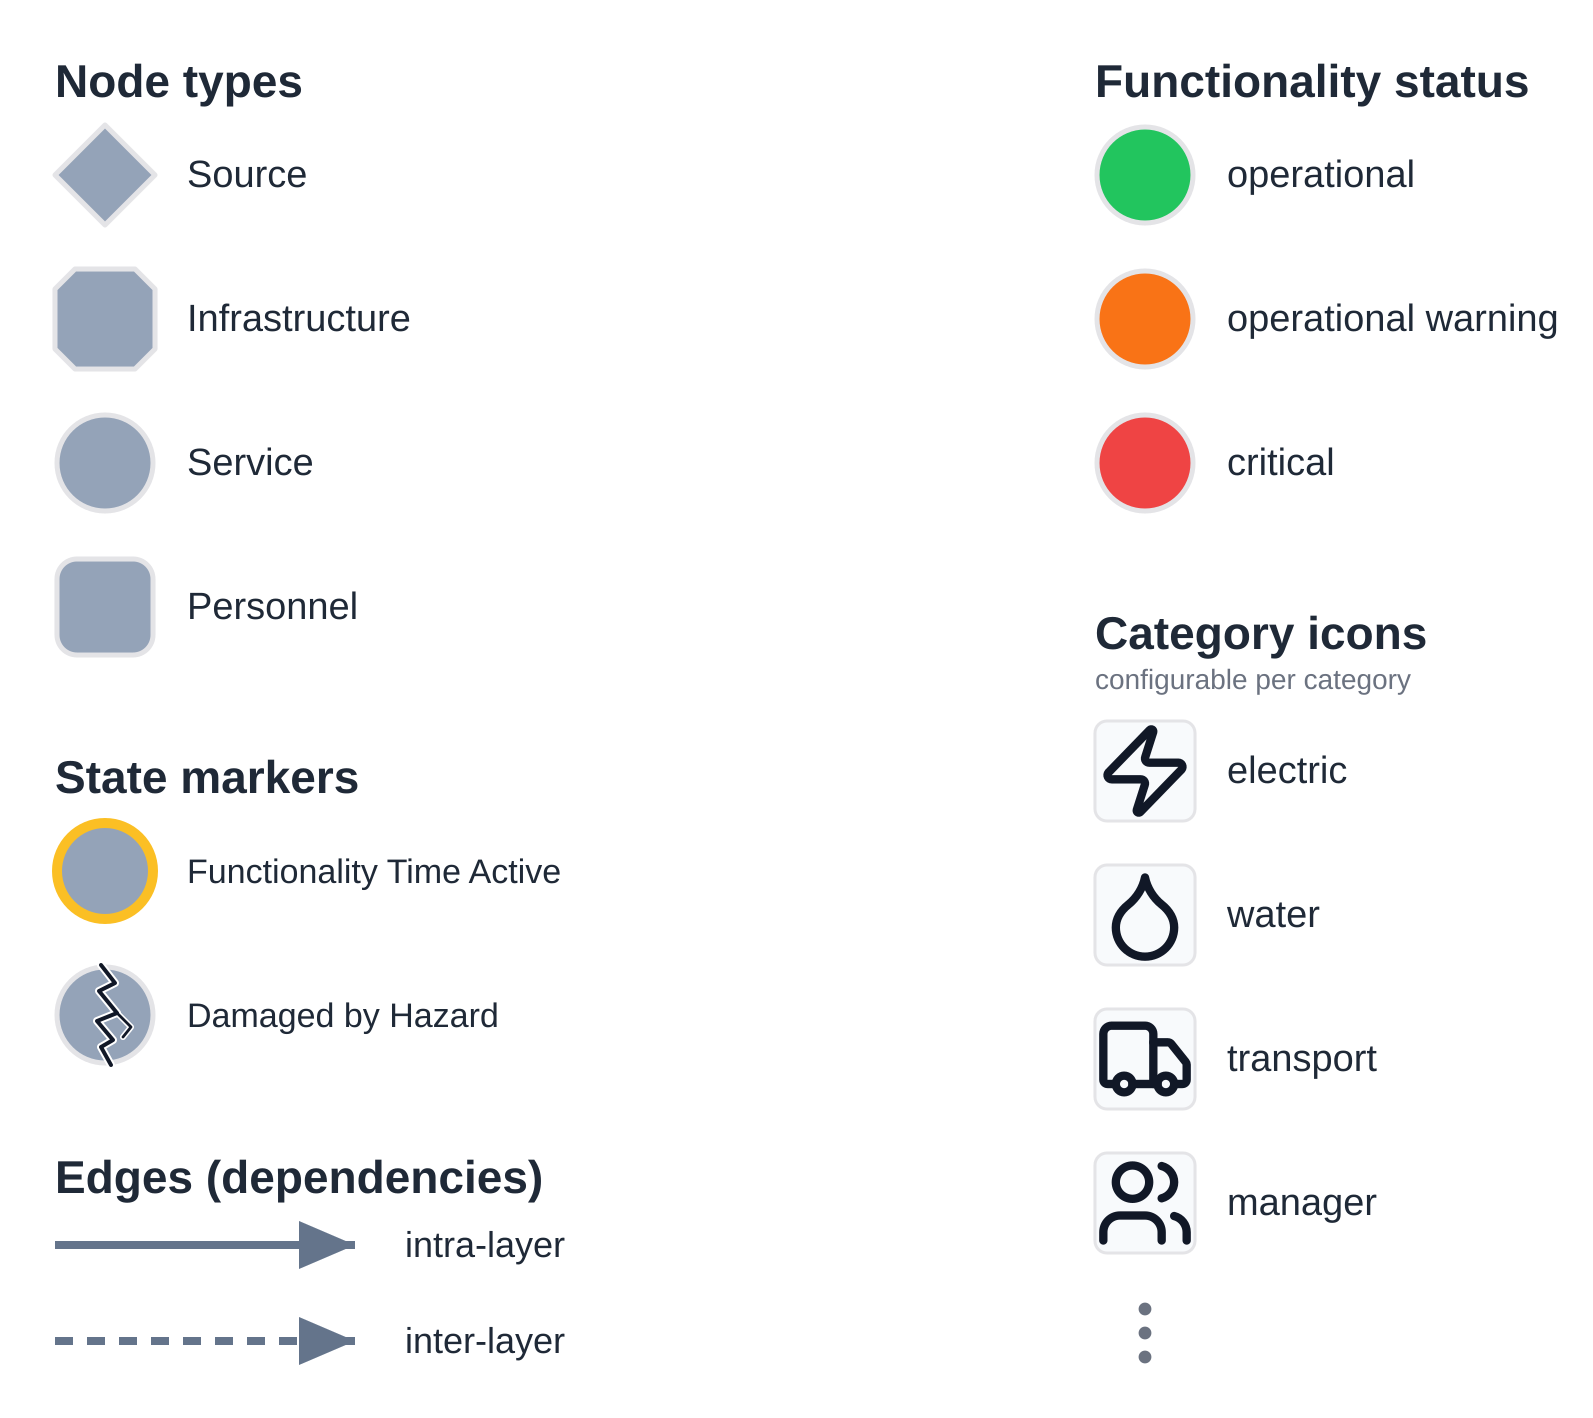
\includegraphics[width=0.5\linewidth]{Figures/legend_full.png}
  \caption{Legend of the CASCADE network elements. \emph{Node types} are distinguished by shape and \emph{Functionality
  status} by fill colour on the three-level scale (valid also for edges);
  an icon inside each node marks its \emph{category} (electric, water, transport,
  managerial, \dots). An amber border flags a node holding on backup (Functionality Time active), and a crack marks direct
  hazard damage. Directed edges denote dependencies (tail \emph{provides to} head);
  dashed edges cross layers (inter-canvas).}
  \label{fig:map_legend}
\end{figure}

\begin{figure}[H]
  \centering
  \includegraphics[width=0.9\linewidth, clip]%
      {Figures/Electrical.png}
  \caption{Electrical layers: \texttt{Electric Source} feeding eight substations in a partially meshed ring topology.
  The source carries a \texttt{manager} dependency on the
  \texttt{electric Operator}.}
  \label{fig:layers_electric}
\end{figure}

\paragraph{Water subsystem}
Two sources provide water:
\texttt{Fauglis water Source} ($\mathit{supply\_capacity} = 45$) and
\texttt{Local water Source} ($\mathit{supply\_capacity} = 10$),
for a total nominal capacity of 55 units.
Distribution is handled by six intermediate junction nodes:
\texttt{San Marco water}, \texttt{Palmanova Porta Ud}, \texttt{Palmanova Porta Cividale}, \texttt{Joint est water}, \texttt{Jalmicco water}, and
\texttt{Industrial water}.
Like the electric subsystem, the \texttt{water} category is typed
\texttt{SourceToDemands}; the engine applies flow-based allocation where, at first, we assume no prioritisation can be executed by the \texttt{water Operator} (by default, topologically-near demands are fulfilled first). \texttt{Fauglis water Source} carries a power dependency (dependency level~2) because its pumping station relies on electricity.

\begin{figure}[H]
  \centering
  \includegraphics[width=0.9\linewidth, clip]%
      {Figures/Water.png}
  \caption{Water layers: two sources (\texttt{Fauglis}, capacity~45;
  \texttt{Local}, capacity~10) feeding six distribution junctions
  and demand endpoints with flow-based priority allocation.}
  \label{fig:layers_water}
\end{figure}

\paragraph{Transport subsystem}
Modelled as a \texttt{Requisite} category, encoding physical accessibility
rather than volumetric flow.
The network includes three regional access points (\texttt{Cividale Access},
\texttt{Udine Access}, \texttt{Aquileia access}),
a southern routing junction (\texttt{Sud-Ovest Joint}),
per-municipality local connectors (\texttt{Palmanova transport},
\texttt{Sottoselva transport}, \texttt{Jalmicco transport},
\texttt{San Marco transport}, \texttt{Industrial transport},
\texttt{joint est transport}),
and the structurally sensitive bottleneck \texttt{Underpass San Marco}.
Functionality degradation reflects loss of access routes rather than capacity constraints.

\begin{figure}[H]
  \centering
  \includegraphics[width=0.9\linewidth, clip]%
      {Figures/Transport.png}
  \caption{Transport layers modelled as a \texttt{Requisite} category.}
  \label{fig:layers_transport}
\end{figure}

\paragraph{Managerial layer}
Four organisational nodes (\texttt{water Operator}, \texttt{electric Operator}, \texttt{transport Operator}, \texttt{civil protection Operator};
all \texttt{node\_category = manager}) represent the entities responsible
for managing the respective services and coordinating emergency response.
\texttt{civil protection Operator} acts as the coordination hub, exchanging
status signals with each of the other three operators.
Edges from each operator to the infrastructure it manages encode digital control dependencies (e.g.\ \texttt{electric Operator}
$\to$ \texttt{Electric Source}; \texttt{water Operator} $\to$ \texttt{Fauglis water Source}): if an operator degrades, the service it manages degrades with it.

\begin{figure}[H]
  \centering
  \includegraphics[width=0.6\linewidth, clip]%
      {Figures/Managerial.png}
  \caption{Managerial layers: four organisational operators
  (\texttt{civil protection Operator} as coordination hub,
  plus \texttt{water}, \texttt{electric}, and \texttt{transport} operators).}
  \label{fig:layers_Managerial}
\end{figure}

\paragraph{Service layer}
Seven demand endpoints are distributed across three categories.
Four municipal nodes (\texttt{Palmanova}, \texttt{San Marco},
\texttt{Sottoselva}, \texttt{Jalmicco}; category \texttt{city})
represent urban settlements.
Two essential-service nodes (\texttt{Hospital}, \texttt{Civil Protection}) represent high-importance facilities.
One major economic node (\texttt{Industrial}) represents the industrial district.
Economic relevance is encoded through
\texttt{cost\_of\_disservice\_per\_day}:
\texttt{Hospital} and \texttt{Palmanova} (100\,000~€/day);
\texttt{Sottoselva}, \texttt{San Marco}, \texttt{Jalmicco},
\texttt{Civil Protection}, and \texttt{Industrial} (10\,000~€/day).

\begin{figure}[H]
  \centering
  \includegraphics[width=0.9\linewidth, clip]%
      {Figures/Service.png}
  \caption{Service layers: four city nodes, two essential-service nodes
  (\texttt{Hospital}, \texttt{Civil Protection}), and one economic node
  (\texttt{Industrial}).}
  \label{fig:layers_service}
\end{figure}

\begin{figure}[H]
  \centering
  \includegraphics[width=0.9\linewidth, clip]%
      {Figures/all.png}
  \caption{Merged view of all five layers, showing the full interdependency graph with dashed cross-layers.}
  \label{fig:layers_all}
\end{figure}

\paragraph{Hazard and disservice vulnerability encoding}
Three stressor events are configured for this case study:
\texttt{strong\_earthquake} (seismic hazard), \texttt{flood}
(hydrological hazard), and \texttt{digital\_attack} (cyber disservice).
Vulnerability is encoded as an integer level per node (and per edge):
0 means no vulnerability (default); 1 implies a minor effect (element degrades to
\texttt{operational\_warning}); 2 implies significant exposure (element
degrades to \texttt{critical}).
The vulnearability assignments are derived from expert knowledge of each system or validated via data-driven hazard simulations when available.
Table~\ref{tab:vulnerability} summarises the non-zero vulnerability entries.

\begin{table}[H]
\centering
\caption{Non-zero vulnerability levels by element and stressor. Levels: 1 = minor exposure (element degrades to \texttt{operational\_warning}); 2 = significant exposure (element degrades to \texttt{critical}); elements/stressor pairs not listed have vulnerability level 0 (no effect).}
\label{tab:vulnerability}
\small
\begin{tabular}{lccc}
\toprule
\textbf{Element} & \textbf{Strong EQ} & \textbf{Flood} & \textbf{Digital attack} \\
\midrule
\texttt{Sud electric}          & 2 & -- & -- \\
\texttt{Local water Source}          & 2 & -- & -- \\
\texttt{Cividale Access}             & 2 & -- & -- \\
\texttt{Aquileia access}             & 1 & -- & -- \\
\texttt{Sottoselva} (city)           & 1 & -- & -- \\
\texttt{San Marco} (city)            & 1 & -- & -- \\
\texttt{Palmanova} (city)            & 1 & -- & -- \\
\texttt{Jalmicco} (city)             & 1 & -- & -- \\
\texttt{Joint est water}             & -- & 2 & -- \\
\texttt{San Marco water}             & -- & 1 & -- \\
\texttt{Underpass San Marco}         & -- & 2 & -- \\
\texttt{electric Operator}           & -- & -- & 2 \\
\midrule
Edge: Sottoselva transport$\leftrightarrow$ Jalmicco transport  & -- & 1 & -- \\
Edge: joint est transport$\leftrightarrow$ Jalmicco transport  & -- & 1 & -- \\

\bottomrule
\end{tabular}
\end{table}

\subsubsection{Illustrative rules and dependency semantics}
\label{subsubsec:case_rules}

Three custom rules override or supplement default propagation logic to encode
context-specific operational resilience strategies and domain expertise.

\paragraph{Nested intercategorical redundancy rule (Jalmicco node)}
Proximity to \texttt{Civil Protection} enables rapid mitigation of electric
and water disruptions provided transport access is maintained.
Formally: the node degrades only if \emph{both} of the following hold
simultaneously — (i)~transport is impaired, \emph{and} (ii)~one among water
and electric is impaired.
This is modelled through the following intercategorical rule:
\begin{verbatim}
worst_of(
  best_of(Jalmicco electric, Jalmicco transport),
  best_of(Jalmicco water,    Jalmicco transport)
) propagates to Jalmicco
\end{verbatim}

\paragraph{Intracategorical rule (Palmanova transport)}
Palmanova is served by three road access routes.
Unlike a simple redundancy model — where a single open route would keep the
city fully connected — urban traffic demand in this area means that
progressive route closures produce increasing degradation rather than a binary
outcome.
This is captured by an \texttt{average\_of} aggregation rule:
\begin{verbatim}
average_of(Udine Access, Aquileia access, Cividale Access)
  propagates to Palmanova transport
\end{verbatim}
For example, with one route at \texttt{critical} and two at
\texttt{operational}, the propagated proposal yields
\texttt{operational\_warning} ($\lfloor(1+3+3)/3\rfloor = 2$), correctly reflecting a city still reachable but under significant congestion pressure.

\paragraph{Specific guard rule (Fauglis water Source)}
The \texttt{Fauglis water Source} has a power dependency at level~2.
However, an established inter-sectoral communication protocol between the
water and electric operators encodes a preparedness arrangement: coordinated
early intervention prevents the source from degrading as long as both
operators remain functional.
This is modelled as a specific guard rule:
\begin{verbatim}
if water Operator.is_communicating_with_electric_operator is True
and water Operator is operational
and electric Operator is operational
then Fauglis water Source is operational
\end{verbatim}
The first condition reads a custom-defined node attribute of \texttt{water Operator}, encoding whether the inter-sectoral protocol is active. The second and third conditions check the live functionality of both operators in the current propagation round.
When all three hold, the rule intercepts any degradation proposal for
\texttt{Fauglis water Source} and replaces it with \texttt{operational}
(level~3). If either operator degrades (for example, from a digital attack impairing their communication systems), the guard does not fire and the default dependency propagation takes over.


%----------------------------------------------------------------------
\subsection{Hazard and disservice scenarios: three illustrative cascades}
\label{subsec:case_scenarios}

We illustrate CASCADE through three stressors of different origin---a
\emph{strong earthquake} (Scenario~A), a \emph{flood} (Scenario~B), and a \emph{digital attack} (Scenario~C)---selected to exercise complementary engine mechanisms: physical damage, flow allocation, redundancy, time-limited backups, and cross-sector control dependencies. Each is read as an initial event footprint
followed by the propagated fixed-point state, and is accompanied by a step-by-step \emph{Propagation Engine Description} with before/after figures.

\subsubsection{Scenario~A: Strong earthquake — electric and transport collapse}
\label{subsubsec:scenarioA}

A strong earthquake directly degrades elements as described in
Table~\ref{tab:vulnerability}
(vulnerability level~2 $\to$ \textbf{critical};
level~1 $\to$ \textbf{operational\_warning}).
Because the drop in functionality results from physical damage, affected
nodes are shown with a ``cracked'' appearance in
Figure~\ref{fig:scenarioA}.

\noindent\textbf{Propagation Engine Description.}
The degradation of \texttt{Cividale Access} to \textbf{critical} and
\texttt{Aquileia access} to \textbf{operational\_warning} propagates
through the \texttt{average\_of} rule, propagating
\textbf{operational\_warning} to \texttt{Palmanova transport}.
Because both \texttt{Jalmicco transport} (whose bridge is
seismically vulnerable) and \texttt{Jalmicco water} are degraded
simultaneously, the inter-categorical rule described in
Section~\ref{subsubsec:case_rules} cannot compensate, and
\texttt{Jalmicco} drops to \textbf{critical}.

The damaged \texttt{Sud electric} station cuts power to \texttt{San Marco} and \texttt{Industrial}: \texttt{San Marco}, with only a partial power dependency, degrades just to \textbf{operational\_warning}, whereas \texttt{Industrial}
drops to \textbf{critical}.
\texttt{Local water Source} at critical reduces total water supply from
55 to 45 (only \texttt{Fauglis} remains), stressing the distribution
network: \texttt{Civil Protection} and \texttt{Hospital} engage their
water backups (shown as a yellow ring in Figure~\ref{fig:scenarioA}),
while \texttt{Jalmicco} is cut off.
Despite \texttt{Fauglis water Source} depending on \texttt{Sud electric}, its specific guard rule fires and preserves full functionality.


\begin{figure}[H]
    \centering
    \includegraphics[width=1\linewidth]%
        {Figures/Strong_Earthquake.png}\\[6pt]
    \includegraphics[width=1\linewidth]%
        {Figures/Strong_Earthquake_Propagated.png}
    \caption{Scenario~A (\texttt{Strong Earthquake}): direct impact (top) and state after first propagation step (bottom).
    Degradation of two regional access nodes drives the transport cascade; the damaged \texttt{Sud electric} station triggers a localised power outage while the \texttt{Fauglis water Source} guard rule keeps the primary water supply intact.}
    \label{fig:scenarioA}
\end{figure}

%----------------------------------------------------------------------
\subsubsection{Scenario~B: Flood — water distribution disruption}
\label{subsubsec:scenarioB}

A flood event degrades elements according to their \texttt{flood}
vulnerability levels (level~2 $\to$ \textbf{critical}; level~1 $\to$ \textbf{operational\_warning}).

\noindent\textbf{Propagation Engine Description.}
\texttt{Joint est water} dropping to critical affects supply to
\texttt{Hospital}, \texttt{Civil Protection}, \texttt{Sottoselva}, and \texttt{Jalmicco water}.
\texttt{Hospital} and \texttt{Civil Protection} engage their 48-hour water backups, deferring the critical drop to the intervention window.

With \texttt{Jalmicco water} at critical and \texttt{Jalmicco transport} at \textbf{operational\_warning}, the Jalmicco nested inter-categorical rule fires: transport redundancy partially compensates for the failed water junction, keeping \texttt{Jalmicco} from reaching critical.

On the transport side, \texttt{San Marco transport} at critical does not cascade further thanks to topological redundancy in the access network.
However, \texttt{San Marco water} at \textbf{operational\_warning}
propagates a mild degradation to the \texttt{San Marco} city node.

\begin{figure}[H]
    \centering
    \includegraphics[width=1\linewidth]%
        {Figures/Flood.png}\\[6pt]
    \includegraphics[width=1\linewidth]%
        {Figures/Flood_Propagated.png}
    \caption{Scenario~B (\texttt{Flood}): direct impact (top) and
    state after first propagation step (bottom).
    The flood disables \texttt{Joint est water}, collapsing the eastern water distribution while transport redundancy
    limits cascading effects.
    The Jalmicco nested rule keeps that municipality from being critical despite the water junction failure; \texttt{Hospital}, \texttt{Civil Protection} absorb the disruption via their water backups.}
    \label{fig:scenarioB}
\end{figure}


%----------------------------------------------------------------------
\subsubsection{Scenario~C: Digital attack — cross-sector cascade from
operator failure}
\label{subsubsec:scenarioC}

In Scenario~C a digital attack compromises the supervisory control layer, causing loss of SCADA control over the \texttt{electric Operator}.
No physical infrastructure is damaged: degradation originates entirely
from the loss of remote monitoring and dispatch capability.

\noindent\textbf{Propagation Engine Description.}
With \texttt{electric Operator} unable to exercise dispatch control,
\texttt{Electric Source} degrades to \textbf{critical}, triggering a
major blackout across the network.
\texttt{Fauglis water Source} is not immune: it relies on electric pumps to deliver water reliably to the furthest served urban areas, and
therefore degrades alongside the power supply.
\texttt{Hospital} and \texttt{Civil Protection} absorb the dual
electric and water degradation through their backup systems, entering
Functionality Time while maintaining functionality.
\texttt{Jalmicco} is the only city to remain \textbf{operational},
shielded by its inter-categorical nested rule.
\texttt{San Marco}, owing to its partial service dependencies and social resilience, is not critically impacted by the power loss and continues to receive sufficient water, settling at \textbf{operational\_warning}.

\begin{figure}[H]
    \centering
    \includegraphics[width=1\linewidth]%
        {Figures/Digital_Attack.png}\\[6pt]
    \includegraphics[width=1\linewidth]%
        {Figures/Digital_Attack_Propagated.png}
    \caption{Scenario~C (\texttt{Digital Attack}): directly affected nodes (top) and state after first propagation step (bottom).
    The attack leaves all physical infrastructure intact but disables
    remote dispatch, causing a major blackout that propagates from the
    electric source through the water pumping system.
    \texttt{Hospital} and \texttt{Civil Protection} fall back on
    backup systems; \texttt{Jalmicco} remains operational via its nested rule, while \texttt{San Marco} is only partially impacted.}
    \label{fig:scenarioC}
\end{figure}


%----------------------------------------------------------------------
\subsection{Strategic updates and their effects}
\label{subsec:case_strategic}

To demonstrate how the framework supports strategy evaluation, we compare baseline scenarios with modified versions that implement simple structural or policy-level changes.
In each case, the modification is encoded directly in the project model —by removing a vulnerability entry, adding a guard rule, or adjusting priority weights — and the engine is re-run to compute the updated cascade.

%----------------------------------------------------------------------
\subsubsection{Strengthening the water infrastructure}
\label{subsubsec:strategic_aqueduct}

Floods can cause structural damage to water junctions and increase the
risk of contamination.
Model outputs indicated to stakeholders that \texttt{Joint est water}
warrants priority intervention: it sits in a low-lying area recurrently
exposed to flooding and is the sole supply gateway for
\texttt{Sottoselva}, \texttt{Jalmicco}, \texttt{Civil Protection}, and
\texttt{Hospital}.
The proposed intervention couples physical hardening with the deployment of a SCADA system on strategic junctions and valves, enabling faster fault detection and supporting timely field responses, like hydraulic bypass manoeuvres, preventing disservice.

A key operational outcome is that the existing redundant path through
\texttt{Palmanova} — connecting \texttt{San Marco water} to
\texttt{Joint est water} via an alternative route — is now reliably
exploited even when the direct \texttt{San Marco water} $\leftrightarrow$ \texttt{Joint est water} link is impaired.
Previously available but not structurally leveraged, this alternative path becomes an effective fallback for maintaining service continuity to the eastern essentials under flood conditions, even though \texttt{Jalmicco water} remains unserved. In the model, this intervention is encoded by removing the \texttt{flood} vulnerability entry from \texttt{Joint est water}.

\begin{figure}[H]
  \centering
    \includegraphics[width=1\linewidth]%
      {Figures/Flood_Propagated.png}\\[0.8em]
  \includegraphics[width=1\linewidth]%
      {Figures/Flood_Propagated_after_improvement.png}
  \caption{\textbf{Pre- and post-intervention propagated flood scenario.}
  Before intervention (top, identical to the propagated flood state of
  Figure~\ref{fig:scenarioB}), failure of \texttt{Joint est water}
  collapses eastern water distribution and forces \texttt{Hospital}
  and \texttt{Civil Protection} onto backup systems.
  After intervention (bottom), the hardened junction withstands the
  flood and the redundant path through \texttt{Palmanova} sustains
  continuous service to essential services and \texttt{Sottoselva}.}
  \label{fig:water_pre_post}
\end{figure}

\subsubsection{Prioritising electricity supply to Palmanova}
\label{subsubsec:strategic_electric_priority}


Grid stress events --- prolonged peak demand, partial generation failures,
or upstream transmission faults --- can reduce the effective output of the
\texttt{Electric Source} below the aggregate demand of the regional
network.
Under scarcity, allocation becomes a managed trade-off: grid operators
who retain control over distribution infrastructure may
selectively steer supply to higher-priority feeders to safeguard critical urban loads.

\texttt{Palmanova electric} lacked an explicit priority assignment relative to industrial and peripheral consumers, exposing the city of \texttt{Palmanova} --- a large urban hub
hosting crucial services --- to avoidable degradation under moderate shortage scenarios.
The proposed intervention formalises a preferential load-shedding agreement with the grid operator, ensuring that the Palmanova feeder is served before lower-criticality consumers whenever the \texttt{Electric Source} operates below full capacity.

In the model, this intervention is encoded by increasing the
\texttt{priority} field of \texttt{Palmanova electric}'s electricity dependency.
\begin{figure}[H]
  \centering
    \includegraphics[width=1\linewidth]%
      {Figures/electric_Propagated.png}\\[0.8em]
  \includegraphics[width=1\linewidth]%
      {Figures/electric_propagated_prioritized.png}
  \caption{\textbf{Pre- and post-intervention propagated electric shortage.}
  Before (top) and after (bottom) prioritisation under a moderate \texttt{Electric Source} shortage.
  Raising \texttt{Palmanova electric}'s \texttt{priority} fully satisfies its demand allowing \texttt{Palmanova} city to remain \texttt{operational}. 
  The reallocation of the remaining supply to lower-priority nodes doesn't cause any additional worsening due to the functionality scale granularity of the model.}
  \label{fig:electric_pre_post}
\end{figure}

%----------------------------------------------------------------------
% \subsubsection{Reinforcing Jalmicco transport bridge}
% \label{subsubsec:strategic_bridge}

% In Scenario~A the seismic vulnerability of \texttt{Jalmicco transport}
% (level~2, both the node and the connecting edges) causes it to reach
% \textbf{critical} after a strong earthquake.
% Because the Jalmicco nested rule makes the city's operativity contingent
% on transport access, the collapse of the bridge propagates to
% the city node.

% A structural intervention — seismic intervention of the bridge — is
% encoded by (i)~removing the \texttt{strong\_earthquake} vulnerability
% entry from \texttt{Jalmicco transport}:
% The engine re-propagates the earthquake scenario from this updated
% baseline.
% With \texttt{Jalmicco transport} held at \texttt{operational}, the
% inner \texttt{best\_of} terms in the nested rule both evaluate to 3,
% and the outer \texttt{worst\_of} remains at 3 — Jalmicco city
% \textbf{stays operational} despite the collapse of all three western
% access routes.
% Civil Protection can maintain its governance function in the eastern
% zone, and the hospital backup timeline is unaffected.

% \begin{figure}[H]
%   \centering
%   \includegraphics[width=1\linewidth]%
%       {Figures/Jalmicco_Bridge_Before.png}\\[0.8em]
%   \includegraphics[width=1\linewidth]%
%       {Figures/Jalmicco_Bridge_After.png}
%   \caption{\textbf{Earthquake cascade before and after bridge intervention.}
%   \textbf{Top:} baseline earthquake propagation — \texttt{Jalmicco transport}
%   collapses to \textbf{critical}, triggering the nested rule and driving
%   Jalmicco city to \textbf{critical}.
%   \textbf{Bottom:} post-intervention propagation — seismic vulnerability
%   removed and guard rule added; \texttt{Jalmicco transport} holds at
%   \textbf{operational}, the nested rule keeps Jalmicco city operational,
%   and Civil Protection retains local governance capacity.}
%   \label{fig:jalmicco_bridge}
% \end{figure}

%----------------------------------------------------------------------
% \subsubsection{Water flow priority control}
% \label{subsubsec:strategic_flow}

% In Scenario~C the digital attack reduces \texttt{Fauglis water Source}
% to \textbf{operational\_warning}, cutting effective supply.
% In the baseline model all demand nodes share the same flow priority
% (level~1), so the min-cost max-flow allocator distributes the reduced
% capacity proportionally: \texttt{Jalmicco water} and
% \texttt{Industrial water} both degrade to \textbf{critical}, while the
% hospital and civil protection nodes remain served only because they share
% higher-priority supply paths.

% The strategic update encodes differentiated flow priorities directly on
% the \texttt{water} category dependency profiles of the demand nodes:
% \texttt{Hospital} receives priority~10, \texttt{Civil Protection}
% priority~9, and \texttt{Palmanova} city priority~8; all other demand
% nodes retain their default priority of~1.
% No physical change to the network is required — this represents a
% pure policy decision by the water operator, implementable via valve
% scheduling or SCADA set-point configuration.

% With these priorities the engine preferentially routes available water
% to critical services first.
% \texttt{Hospital} and \texttt{Civil Protection} are fully served
% throughout; \texttt{Palmanova} city retains priority access ahead of
% the industrial and peripheral zones.
% The shortfall is absorbed by lower-priority nodes, a controlled trade-off
% that preserves life-safety services at the expense of industrial and
% non-critical demand.

% \begin{figure}[H]
%   \centering
%   \includegraphics[width=1\linewidth]%
%       {Figures/Water_Flow_No_Control.png}\\[0.8em]
%   \includegraphics[width=1\linewidth]%
%       {Figures/Water_Flow_Control.png}
%   \caption{\textbf{Digital attack water cascade without and with flow
%   priority control (Water layers).}
%   \textbf{Top:} baseline — uniform priorities cause the reduced
%   \texttt{Fauglis} supply to be shared proportionally, leaving
%   \texttt{Jalmicco water} and \texttt{Industrial water} at
%   \textbf{critical}.
%   \textbf{Bottom:} after priority assignment
%   (\texttt{Hospital}~10, \texttt{Civil Protection}~9,
%   \texttt{Palmanova}~8) — critical services are fully served first;
%   the supply shortfall is shifted to lower-priority nodes, preserving
%   life-safety capacity under digital disruption.}
%   \label{fig:water_flow_control}
% \end{figure}


%----------------------------------------------------------------------
\subsection{Centrality versus Shapley: Identifying Neuralgic Nodes}
\label{subsec:case_centrality_shapley}

Finally, we compare traditional topological metrics with the proposed Shapley-based neuralgic node analysis.
We computed:
\begin{itemize}
  \item \textbf{Eigenvector and Betweenness Centrality}, computed with NetworkX (power-iteration eigenvector centrality; shortest-path betweenness) on the directed dependency graph (39 nodes, 93 edges);
  \item \textbf{Approximate Shapley Values ($\hat{\phi}_i$)} using the sampling procedure described in Section~\ref{subsec:shapley}, on nodes only, with coalition size limited to three ($k_{\max}=3$) and $M=800$ permutations, and a uniform (constant) Operativity Index weight, so that each node contributes equally to the score regardless of assigned importance or cost\footnote{On a mid-range laptop this required about a minute; the analysis script (\texttt{CASCADE-backend/scripts/paper\_shapley\_vs\_centrality.py} in the CASCADE repository, run on the case-study model \texttt{CASCADE/samples/public/Palmanova\_Complete.json}) reproduces these exact figures by calling the propagation engine directly.}.
\end{itemize}

\noindent\textbf{Interpretation of results.}
Static topological metrics treat all edges as structurally equivalent connections and therefore cannot distinguish a necessary \emph{dependency} — which propagates failure when it degrades — from a \emph{redundancy} — which absorbs failure and provides resilience.
A further limitation in flow-based networks is the tendency to underestimate source nodes: a source may sit at the periphery of the topology yet be the sole origin of an entire resource, so its structural centrality scores remain modest even though its removal collapses supply entirely.

CASCADE's simulation explicitly encodes these distinctions through categories and node attributes.
As shown in Figure~\ref{fig:shapley_ranking}, Shapley values identify neuralgic nodes by accounting for the operational logic of the system --- flow dynamics, requisite conjunctions, and dependency levels --- whereas centrality metrics reward high connectivity (eigenvector) or topological
bridging (betweenness) regardless of whether those structural positions translate into operational criticality.

To quantify this, we computed Spearman rank correlations between $\hat{\phi}_i$ and each centrality measure across all 39 nodes (Table~\ref{tab:shapley_correlation}). Shapley and eigenvector centrality are weakly \emph{anti}-correlated, at the margin of significance ($\rho=-0.31$, $p=0.05$): eigenvector centrality is dominated by well-connected transport junctions. Shapley and betweenness centrality are instead moderately \emph{positively} correlated overall ($\rho=0.74$, $p<10^{-6}$): in this network, several genuine flow bottlenecks (distribution substations, water junctions) are simultaneously high-betweenness and high-Shapley.
Results are summarised in Table~\ref{tab:shapley_correlation}.

A representative contrast: \texttt{Electric Source} scores highest in Shapley value ($\hat{\phi}=1.38$) because its removal collapses the entire power subsystem, yet it ranks only 36th of 39 in eigenvector centrality and 6th in betweenness --- a peripheral-looking source whose criticality both topological metrics understate.
Conversely, transport bridges such as \texttt{Sottoselva transport} and \texttt{San Marco transport} rank in the top ten of \emph{both} eigenvector and betweenness centrality --- being structurally well-connected junctions --- yet contribute comparatively low marginal Shapley value (17th and 24th respectively), because redundant routing absorbs their failure.

\begin{table}[H]
\centering
\caption{Shapley rank versus centrality rank for representative nodes (39 nodes, $M=800$ permutations, $k_{\max}=3$, uniform weight). Top block: highest Shapley-ranked nodes. Bottom block: nodes ranking in the centrality top~10 whose Shapley rank diverges most.}
\label{tab:shapley_correlation}
\small
\begin{tabular}{lccc}
\toprule
\textbf{Element} & \textbf{Shapley rank ($\hat{\phi}_i$)} & \textbf{Eigenvector rank} & \textbf{Betweenness rank} \\
\midrule
\texttt{Electric Source}        & 1 (1.38) & 36 & 6 \\
\texttt{Fauglis water Source}   & 2 (1.00) & 28 & 3 \\
\texttt{water Operator}         & 3 (0.71) & 30 & 14 \\
\texttt{electric Operator}      & 4 (0.70) & 31 & 11 \\
\texttt{San Marco water}        & 5 (0.67) & 19 & 1 \\
\texttt{Sud electric}           & 6 (0.60) & 33 & 2 \\
\midrule
\texttt{Sottoselva transport}   & 17 (0.20) & 4 & 4 \\
\texttt{San Marco transport}    & 24 (0.17) & 6 & 10 \\
\texttt{Aquileia access}        & 23 (0.18) & 1 & 7 \\
\bottomrule
\end{tabular}
\end{table}

\paragraph{From rankings to decisions}
Read together, these indices support complementary decisions. The Shapley ranking answers ``where does scarce hardening budget buy the the most continuity in essential service delivery?'': its values are marginal contributions to Operativity loss, so a shortlist of high-$\hat{\phi}_i$ elements pinpoints where reinforcement, redundancy, or backup investment most reduces cascading impact. 
Moreover, Shapley values share a common, interpretable unit --- fractional Operativity loss --- so they are directly comparable in magnitude: an element with twice the $\hat{\phi}_i$ contributes twice the marginal operativity loss, enabling straightforward prioritisation against an intervention budget. The nodes where the two views \emph{disagree} are the actionable signal: a structurally central node with comparatively low Shapley value (e.g.\ \texttt{Sottoselva transport}, \texttt{San Marco transport}) reveals effective redundancy where mitigation would be misdirected, whereas a peripheral node with high Shapley value (e.g.\ \texttt{Electric Source}) flags a hidden single point of failure that topological screening overlooks.
Eigenvector centrality diverges from Shapley value systematically in this network (negative overall correlation). Centrality thus serves as a fast first pass, while the Shapley analysis refines it with operational logic: the elements where the two rankings diverge are exactly those where topology-only screening is most likely to misjudge operational risk. 
\begin{figure}[htbp]
    \centering
    \includegraphics[width=1\linewidth]%
        {Figures/Shapley_uniform.png}
    \caption{Operationally relevant ranking using approximate Shapley values (darker colour indicates higher value), nodes only (Section~\ref{subsec:case_centrality_shapley}).
    By accounting for the knowledge-driven propagation engine, the ranking surfaces the \texttt{Electric Source} as the most neuralgic element --- an operationally decisive node that both topological metrics below rank only modestly.}
    \label{fig:shapley_ranking}
\end{figure}

\begin{figure}[htbp]
    \centering
    \includegraphics[width=1\linewidth]%
        {Figures/Betweenness.png}
    \caption{Betweenness centrality ranking (darker colour indicates higher value; shortest-path betweenness on unweighted directed graph).
    Overall it agrees moderately with the Shapley ranking ($\rho=0.74$, Table~\ref{tab:shapley_correlation}), as several genuine flow bottlenecks are also topological bridges.}
    \label{fig:betweenness}
\end{figure}

\begin{figure}[htbp]
    \centering
    \includegraphics[width=1\linewidth]%
        {Figures/Eigenvector.png}
    \caption{Eigenvector centrality ranking (darker colour indicates higher value; power-iteration eigenvector centrality on the directed, unweighted graph).
            It elevates well-connected transport hubs.}
    \label{fig:eigenvector}
\end{figure}


\section{Discussion}
\label{sec:discussion}

\subsection{Methodological contributions}
\label{subsec:methodological_contributions}
The framework makes three core methodological contributions that directly address the gaps and research questions outlined in Sections~\ref{sec:intro} and~\ref{sec:litreview}.

\paragraph{First, a functionality-status propagation engine grounded in operational knowledge}
The propagation algorithms model how operativity degrades in interdependent networks through dual mechanisms: a capacity-based max-flow allocation for \emph{SourceToDemands} categories, and a category-aware logical worsening for necessary dependencies. By encoding dependency levels, backup behaviours, and organisational practices as explicit rules and priority values, the framework enables systematic cascade analysis even under severe data scarcity. This directly addresses RQ1 by modelling cross-sector interdependencies through institutional constraints and dispersed operational knowledge.

\paragraph{Second, a tractable Shapley-based approach to neuralgic node identification}
Building on cooperative game theory, the framework adapts Shapley values to quantify each node's marginal contribution to system-wide operativity loss across multiple failure coalitions. While combinatorial complexity has historically limited Shapley-based methods in infrastructure studies, this approach achieves tractability through user-configurable constraints (e.g., time limits, coalition size caps, and sampling strategies). As illustrated in Section~\ref{subsec:case_centrality_shapley}, this propagation-based approach reveals behaviours and effects that standard topological measures fail to capture.

\paragraph{Third, a compositional network-of-networks modelling paradigm}
The framework operationalises a compositional approach in which subsystems (e.g., power, water, digital) are modelled independently by their respective stakeholders and subsequently linked via explicit interfaces. The compositional structure supports incremental refinement, rapid strategic update (both structural and organisational), and the aggregation of dispersed expertise. Coupled with an intuitive rule system, it addresses the "siloed versus integrated representation" gap, responding to RQ2 and RQ3 by framing stress-testing as a structured, participatory learning activity.


\subsection{Practical implications for disaster risk reduction}
\label{subsec:practical_implications}
The framework's design directly addresses the practical and governance challenges faced by emergency management agencies, infrastructure operators and decision makers.

Rapid modelling capabilities (allowing models to be built in days and updated in hours) make the software ideal for tabletop exercises, preventive action prioritisation, preparedness workshops, and dynamic post-event assessments. Rather than requiring exhaustive historical data, users encode existing operational understanding, which the engine then systematically propagates. 

Explicit representation of interdependencies provides a structured methodology to uncover cross-sector dependencies that remain implicit or undocumented. By visualizing these links, the framework supports shared situational awareness and strengthens intersectoral safety and governance by paving a shared common understanding. It highlights critical gaps where redundancies and contingency plans are lacking.

Furthermore, economic loss estimation translates operativity analysis into metrics essential for budget authorities. By associating cost-of-disservice estimates with service components, decision-makers can perform strategic cost--benefit comparisons, weighing the economic impacts of hazard-induced disruptions against the costs of system hardening or operational revisions. 

Finally, the framework aims to broaden access to infrastructure analysis. Traditional high-fidelity simulations often require intermediary technical experts. By utilising a graphical interface and an accessible modelling approach, CASCADE is designed to enable more direct engagement by stakeholders, operators and domain experts. This proactive approach is intended to shift disaster preparedness from reactive, post-event learning toward collaborative, anticipatory modelling.



\subsection{Limitations and constraints}
\label{subsec:limitations}
The framework fills a specific niche in the DRR toolkit; its scope and constraints must be clearly defined.

\paragraph{Not a high-fidelity physical simulation}
The system does not simulate detailed physical processes from "scratch," nor does it consider stochastic failure mechanisms or agentic behaviours. It aggregates and formalises existing operational knowledge from experts or information from existing simulations rather than discovering dynamics from first principles. Hence, it should not be adopted for designing new systems.


\paragraph{Need for technical literacy and facilitation}
Though highly accessible, the software requires users to conceptualise systems via networks and to understand the modelling process. We expect that stakeholders and decision makers may require facilitation.

\paragraph{Limited validation}
The framework is currently validated on synthetic demonstrations (Section~\ref{sec:case}) as proof-of-concept. Empirical validation against observed disaster outcomes, retrospective analyses, and longitudinal field deployments remains necessary.

% \paragraph{Undeveloped geographical interdependencies}
% The current implementation focuses on functional interdependencies, with limited spatial modelling of co-location risks. While the hazard customizable design allows it, comprehensive spatial modelling would require integrating distinct hazard footprints and proximity-based co-failure mechanisms.

\subsection{Future research directions}
\label{subsec:future_work}
Future iterations will expand the framework's methodological scope and practical applications.

\paragraph{Explore Applications}
The CASCADE capability to aggregate information enables the modelling of very different organisations at varying levels of granularity. Application examples may be considered from internal hospital services \cite{Grimaz2021}, to the national-level critical utilities \cite{Liu2017} and supply chains \cite{khakifirooz_assessing_2025} resilience analysis, from humanitarian logistics \cite{Liao2023} to complex multi-agency coordination during large-scale evacuations \cite{Harris2021}.

\paragraph{Integration with real-time data}
Integrating CASCADE with sensor networks and SCADA systems would enable real-time operativity assessment during evolving emergencies. As sensors detect degradation, the software could dynamically update functionalities, transitioning CASCADE from a proactive help into an active operational decision aid.

\paragraph{Automated generation of strategic mitigation updates}
Beyond assessing existing vulnerabilities, the framework can be extended to proactively recommend structural and procedural interventions. By coupling the functionality-status propagation engine with search algorithms or heuristics, future iterations could automatically evaluate numerous changes to propose meaningful updates (e.g., targeted redundancies, backups). 

% \paragraph{Propagation-based recovery sequence optimization}
% Future research may address the temporal dynamics of post-disaster recovery. The propagation engine could, in principle, be adapted to simulate reverse-cascades (only improving functionality), evaluating alternative repair sequences to optimize the restoration of interdependent services under logistical constraints. By quantifying how the reactivation of specific neuralgic components propagates positive functionality through the network, this approach will provide actionable, phased recovery schedules that reduce system downtime.

\paragraph{Cross-network comparability via propagation-based metrics}
Finally, another promising avenue is leveraging the propagation engine to extract interpretable metrics that facilitate the comparison among different independent networks. Currently, the framework's Shapley value analysis excels at identifying neuralgic components by comparing nodes contributes within a single system, but the raw numerical outputs lack the intrinsic meaning required for cross-system benchmarking. Future research can focus on exploring propagation-based metrics also for other goals, such as clusterization techniques.

\section{Conclusion} \label{sec:conclusion} Climate-induced hazards and cascading failures represent escalating global challenges, demanding decision-support tools that bridge the gap between theoretical understanding and practical implementation. This paper introduced CASCADE (Customizable Assessment of System Cascades And Dependency Effects), a compositional framework designed to enable rapid, collaborative operativity assessment of interdependent entities, particularly in resource-constrained disaster risk reduction contexts and in the preparedness phase for intersectoral safety enhancement.

The work addressed three core issues. First, it demonstrated how cross-sector interdependencies can be modelled systematically even when formal quantitative data are scarce, utilising a compositional network-of-networks paradigm. This approach enables multi-stakeholder collaboration, allowing diverse organisations to independently encode tacit operational knowledge and seamlessly integrate their subsystems into a shared model of cascading dynamics. Second, it addressed the need for decision-support tools to expand operators' understanding rather than acting as passive, black-box calculators. By making implicit assumptions explicit, the modelling process itself serves as an active learning environment that forces the systematic consideration of dependencies, reveals blind spots, and builds user intuition regarding plausible failure sequences. 
Third, it provided a mechanism for rapid stress-testing under diverse hazard scenarios to support proactive governance. By combining functionality-status propagation with an adapted Shapley value analysis, the framework allows stakeholders to interactively explore "what-if" situations, evaluating hardening measures or joint failures—to proactively assess system operativity, thereby guiding strategic investment and anticipatory preparedness.

The realistic demonstration in Section~\ref{sec:case} illustrated the framework's capability to generate concrete decision-support outputs for disaster preparedness. Notably, the framework translates operativity analysis into financial metrics via cost-of-disservice estimates, enabling budget authorities to perform strategic cost--benefit comparisons. The tool's low data requirements, rapid modelling, and inherently instructive process are intended to support bottom-up disaster risk reduction, helping to broaden access to operativity analysis.

While CASCADE fills a crucial niche in the disaster toolkit, its operational constraints must be acknowledged. It is not a high-fidelity physical simulation discovering dynamics from first principles and requires domain knowledge for meaningful modelling. Furthermore, the software relies on synthetic demonstrations, highlighting the need for future empirical validation.

Ultimately, CASCADE represents not just a software tool, but a shift toward a complementary paradigm: knowledge modelling alongside data-intensive simulation. This approach recognises that operational expertise is itself valuable, overlooked information, that model building can be inherently instructive and participatory, and that rapid insights from structured knowledge often provide more decision value than incomplete but precise predictions.

\section*{Ethics statement}
This work did not involve a formal human-subjects research protocol. Vulnerability levels and network parameters for the case study (Section~\ref{sec:case}) were informed by publicly available infrastructure data, the authors' territorial knowledge, and brief, informal, non-identifying feedback from infrastructure operators; no personal or identifiable data were collected, and no animal subjects were involved.

\section*{CRediT authorship contribution statement}
Cristian Curaba: Conceptualization, Investigation, Methodology, Software, Formal analysis, Writing – original draft, Visualizations.
Fabio Zorzini: Conceptualization, Validation, Visualizations, Writing – review \& editing.
Stefano Grimaz: Supervision, Conceptualization, Writing – review \& editing.

\section*{Funding}
This research did not receive any specific grant from funding agencies in the
public, commercial, or not-for-profit sectors.

\section*{Declaration of competing interest}
The authors declare that they have no known competing financial interests or personal relationships that could have appeared to influence the work reported in this paper.

\section*{Data availability}
The synthetic case-study data and the CASCADE software are available at\newline \href{https://github.com/Cristian-Curaba/CASCADE}{https://github.com/Cristian-Curaba/CASCADE}. The case-study model of Section~\ref{sec:case} is \texttt{CASCADE/samples/public/Palmanova\_Complete.json} (with \texttt{\_water\_improvement} and \texttt{\_electric\_priority} variants for the strategic updates of Section~\ref{subsec:case_strategic}), and the file \texttt{docs/papers.md} in the repository maps each section and figure of this paper to the source file that implements or reproduces it.

\section*{Declaration of generative AI and AI-assisted technologies in the manuscript preparation process}
During the preparation of this work the author(s) used Claude to improve language and readability. After using this tool, the author(s) reviewed and edited the content as needed and take full responsibility for the content of the publication.

\newpage
\bibliographystyle{elsarticle-num}
\bibliography{cas-refs}


\end{document}